
\begin{figure}[htbp]%#1
\begin{center}
%\includegraphics[width=13.4cm,clip=true,bb=-100 -40 730 850]{./figures_llg/CLASTOF.ps.gz}
\includegraphics[width=16cm,clip=true,bb=100 400 930 1300]{CLASTOF.ps.gz}
\end{center}
\caption{CLASTOF.ps.gz.
The preliminary design of  CLAS Central TOF detector  at 12GeV.
\label{barrel}}
\end{figure}
\clearpage


\begin{figure}[htbp]%#11
\begin{center}
%\includegraphics[width=13.4cm,clip=true,bb=-100 -40 730 850]{./figures_llg/CLASTOF.ps.gz}
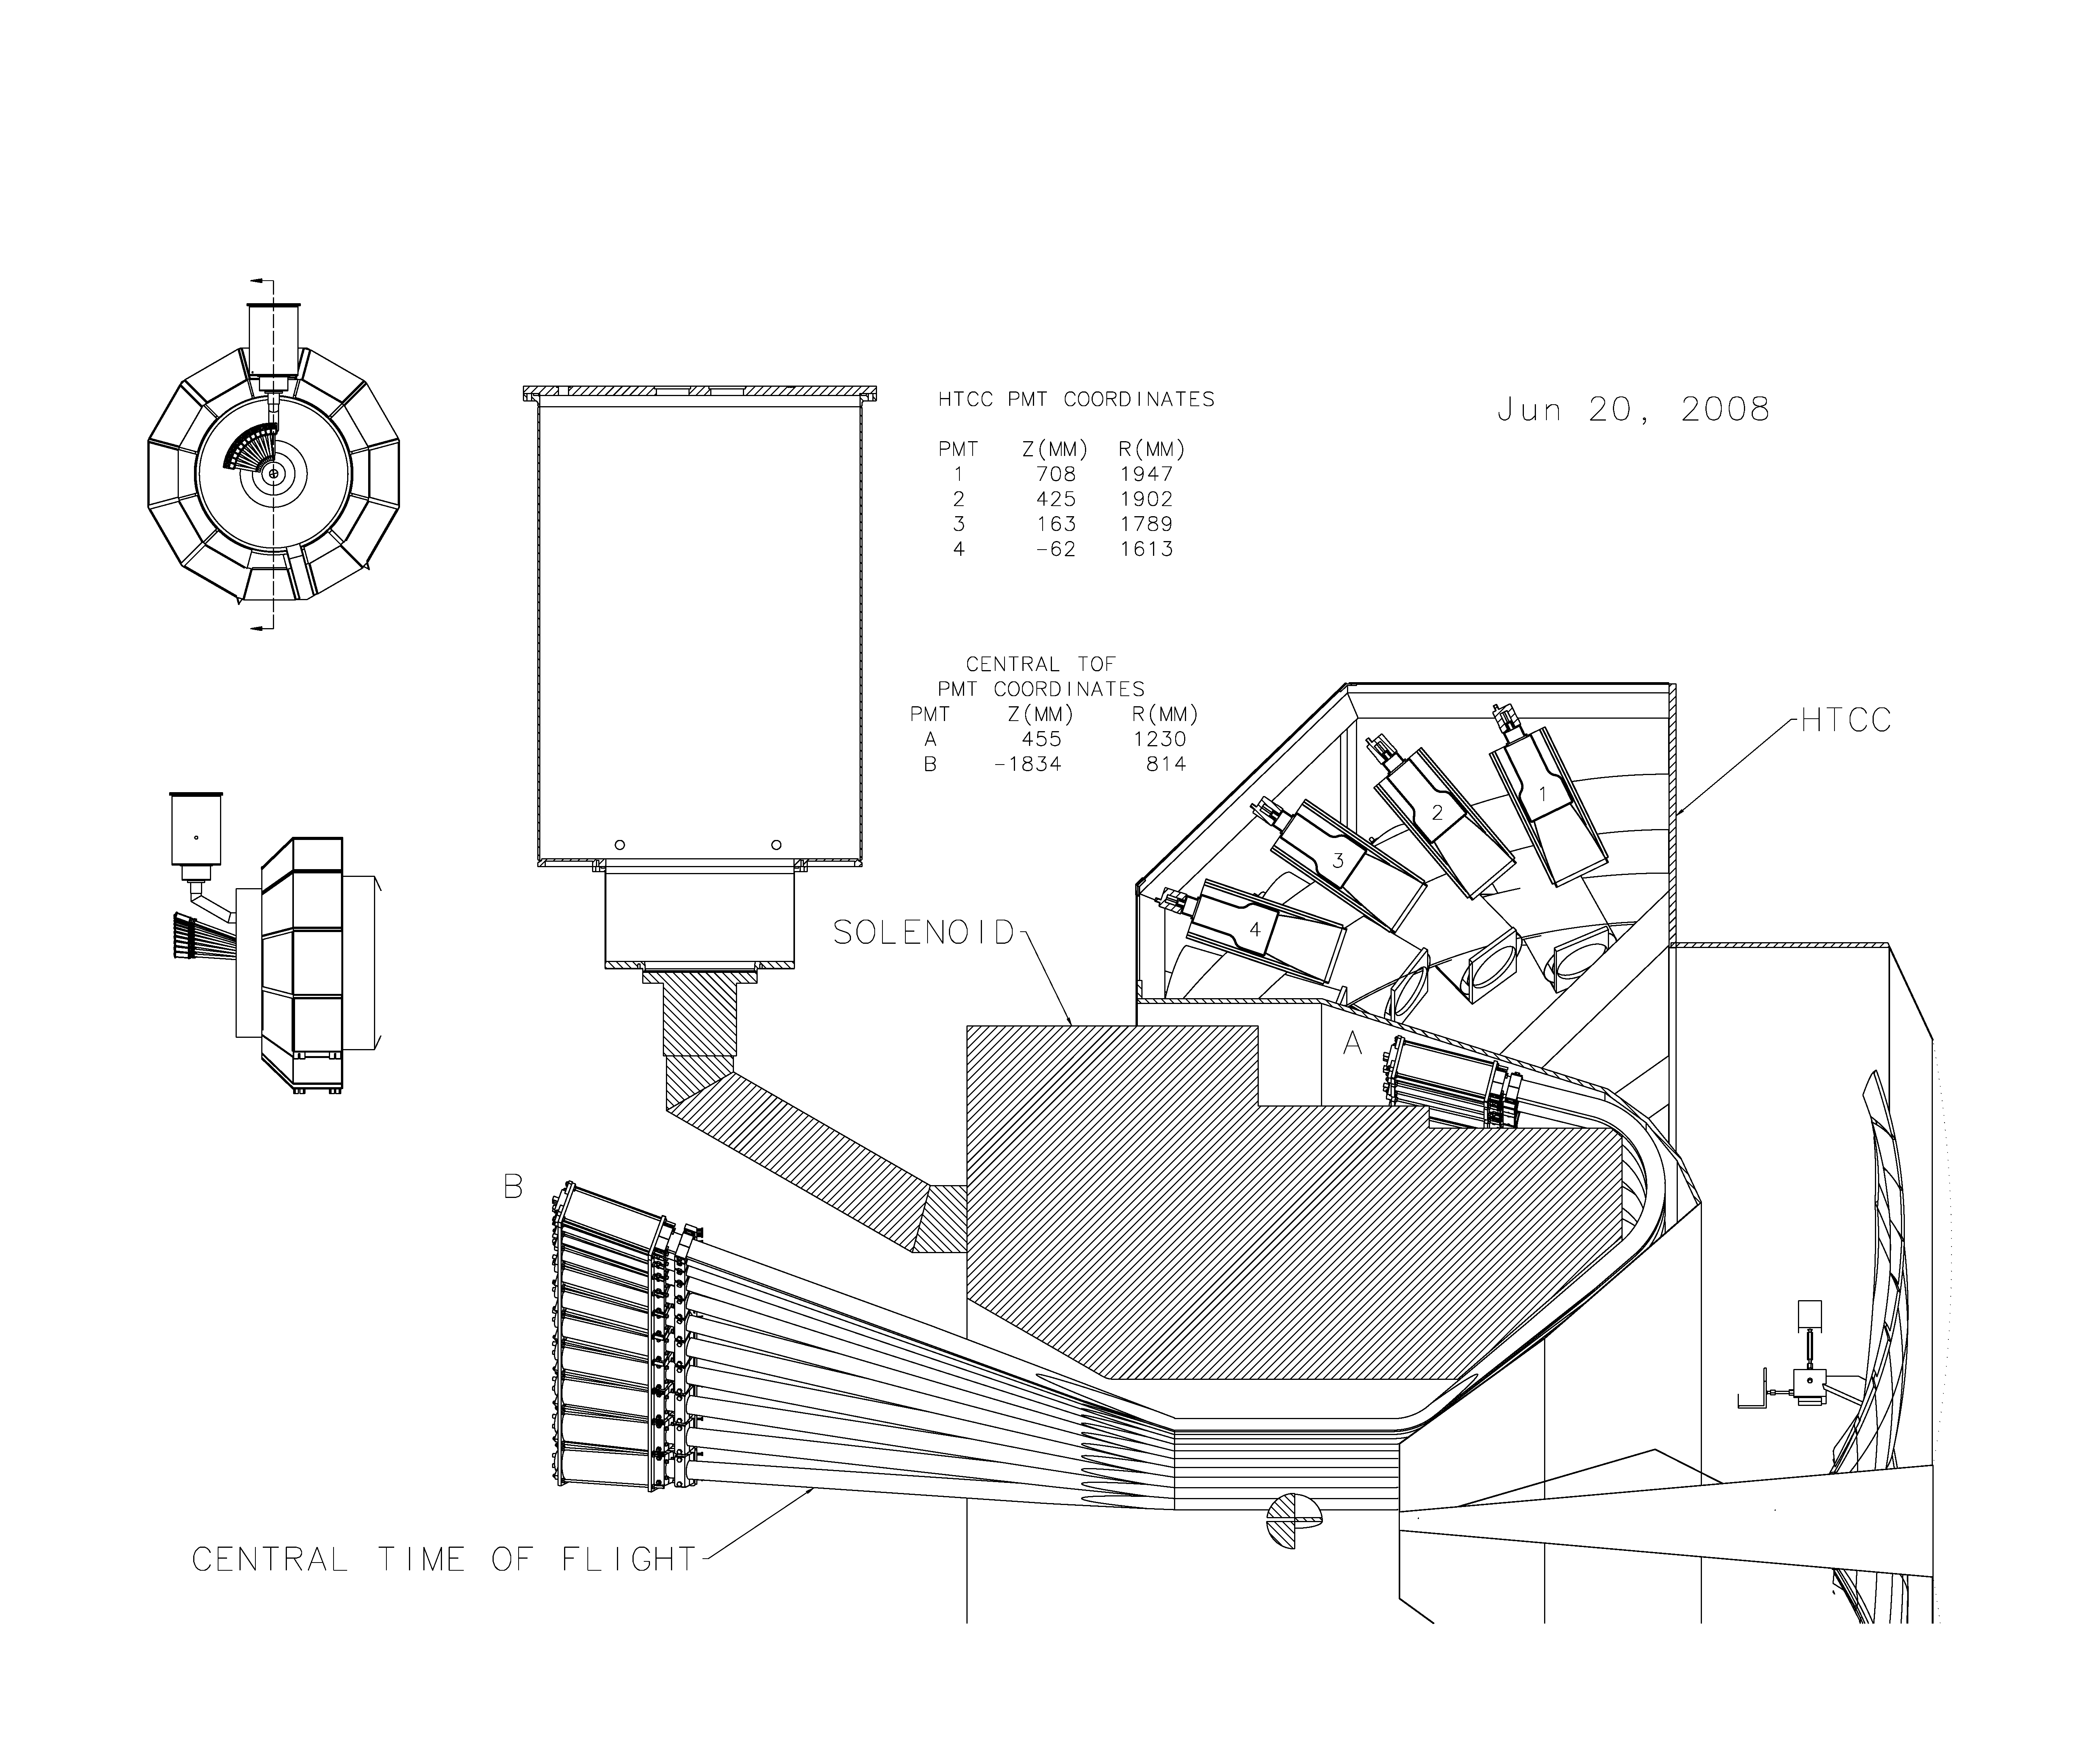
\includegraphics[width=17cm,clip=true,bb=100 600 2800 2000]{HTCC_CTOF_STUDY_060507_WRAP.ps.gz}
\end{center}
\caption{%CLASTOF.ps.gz.
Preliminary layout of the   CLAS Central TOF detector. 
Solenoid is shown as a hatched area. Scintillators form a barrel  66 cm long 
with the inner radius $24.945cm$.
Upstream and downstream,   light guides 
$50mm$ in diameter have a pitch of $7^o$ and $41^o$ respectively. 
The $1.5-1.7m$ long light guides for conventional PMTs
 may be replaced with $\approx1m$ long  light guides to accommodate 
magnetic field immune photo detectors. With this purpose a room 
 is  organized  at the outer downstream side of the solenoid casing.
The room for the magnetic shielding of the conventional PMTs 
may  be increased.
\label{barrel2}}
\end{figure}
\clearpage

%\begin{figure}[htbp]%#12
%\begin{center}
%%\includegraphics[width=13.4cm,clip=true,bb=-100 -40 730 850]{./figures_llg/mmap1.ps.gz}
%\includegraphics[width=17cm,clip=true,bb=100 600 8800 8000]{mmap1.ps.gz}
%\end{center}
%\caption{Layout of conventional PMTs at the magnetic field map.
% Downstream light guide and corresponding PMT are  shown in wite. For both PMTs the field is of $20T$.
%For magnetic immune photodetectors light guides may be  $/approx 0.8m$ long. The corresponding field 
%is of $ 0.6T$. 
%\label{barrel}}
%\end{figure}
%\clearpage
%%%%%%%%%%%%%%%%%%FIG.2%%%%%%%%%%%%%%%%%%%%%%
\begin{figure}[ht]
\vspace*{0.8cm}
\epsfverbosetrue\epsfxsize=15cm\epsfysize=15cm\epsfbox{mmap1.eps}
\vspace*{0.8cm}
\caption{Location of R2083 photo multipliers and magnetic field map.
         \label{fig:mmap1}}
\end{figure}
%%%%%%%%%%%%%%%%%%%%%%%%%%%%%%%%%%%%%%%%%%%%%
\clearpage


\begin{figure}[htbp]%#2
\begin{center}
%\includegraphics[width=13.8cm,clip=true,bb=-0 -40 720  800]{/home/prof/batourine/knu/publications/rep_llg_fromJLAB/cosmic-6pmtllg_picture.ps.gz}
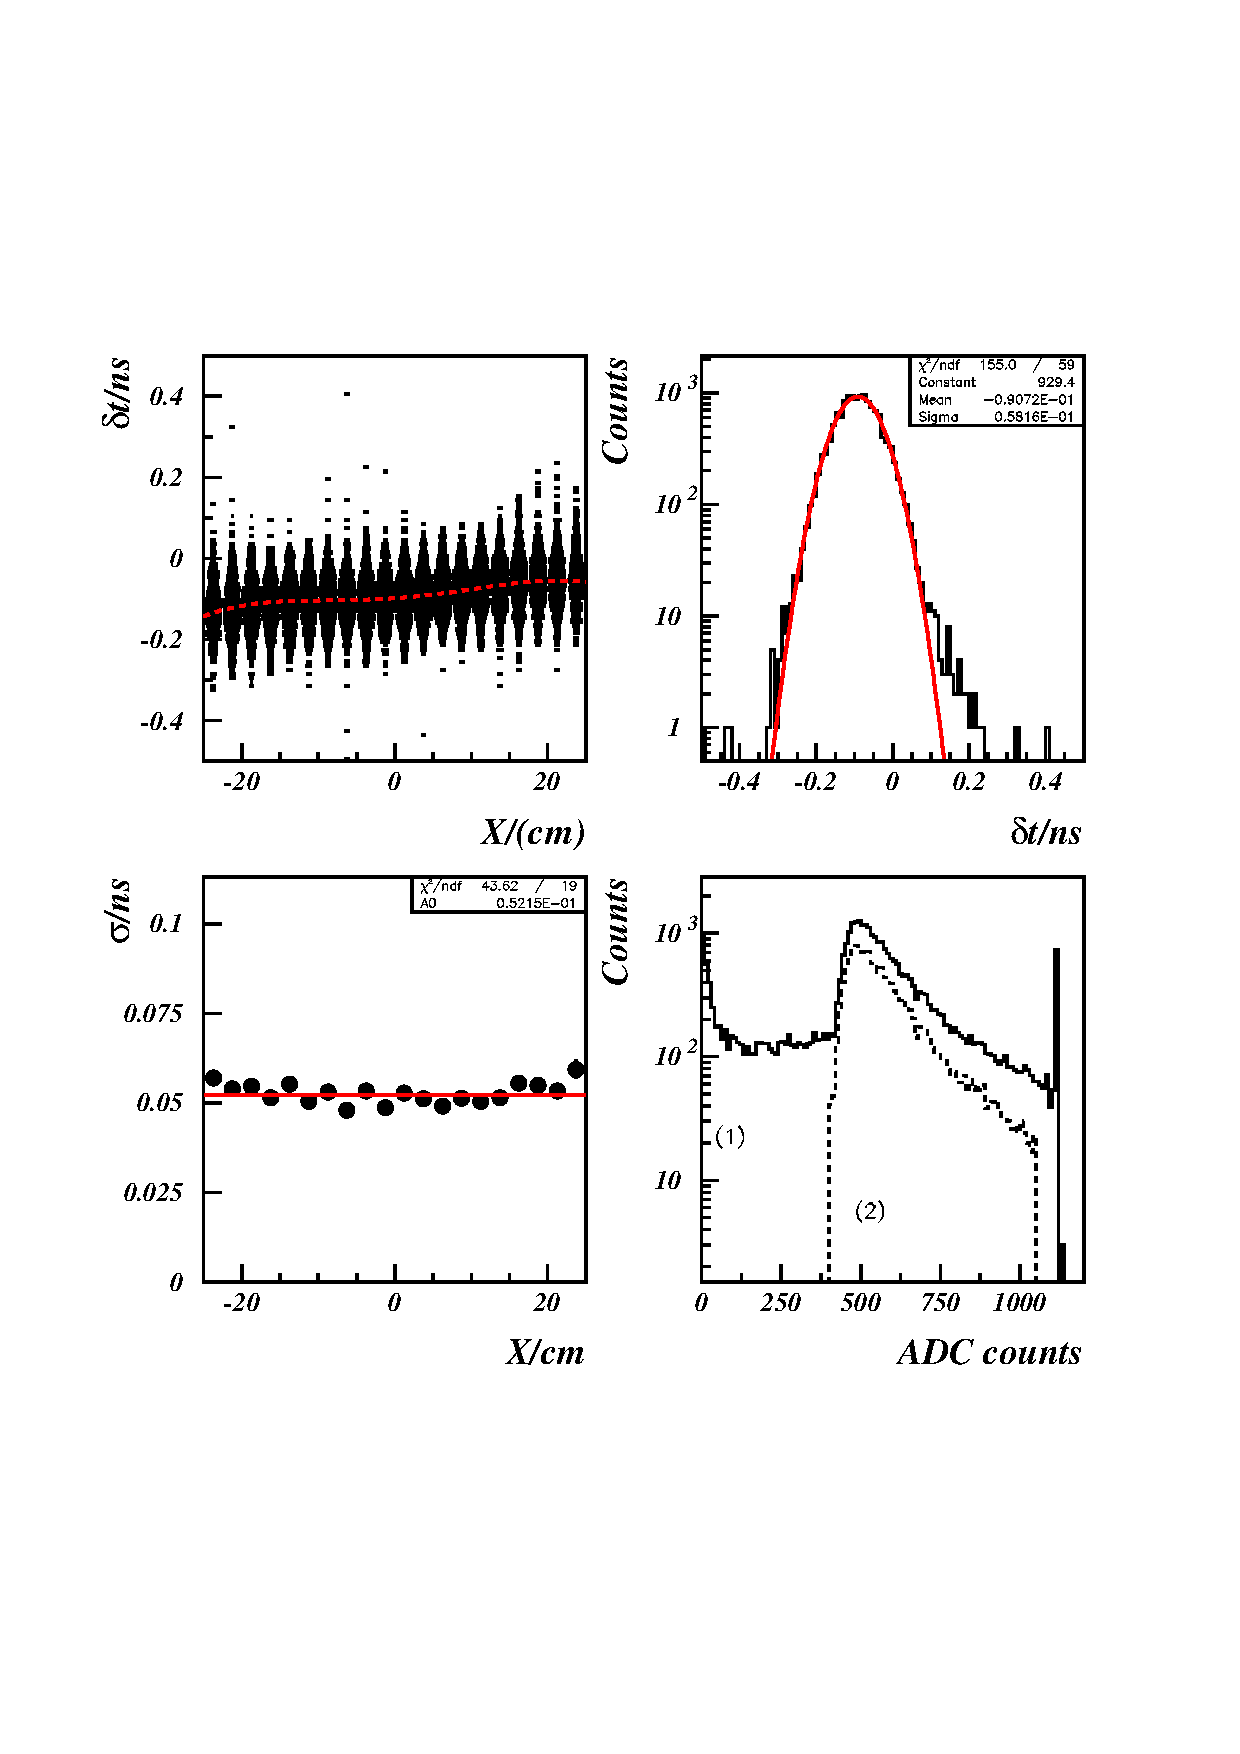
\includegraphics[width=13.8cm,clip=true,bb=20 150 620  720]{cosmic-6pmtnlg_picture.ps.gz}
\end{center}
\caption{%cosmic-6pmtnlg-picture.ps.gz,
Effective time resolution of R2083 PMT($\sigma$)
 in the reference triplet without 
light guides. Panel
1)top-left: scatter plot of residuals vs longitudinal coordinate $x$,
2)top-right: overall distribution of residuals with $\sigma_{R2083}=52.2\pm0.4~ps$, 
3)bottom-left: local $\sigma$ vs $x$,
4)bottom-right:  ADC values. Histogram (1) -raw events, histogram (2) - selected events when $both$ ADC values
are in the  span of this histogram.
\label{nlgres}}
\end{figure}


\begin{figure}[htbp]%#3
\begin{center}
\includegraphics[width=13.8cm,clip=true,bb=20 150 620  720]{cosmic-6pmtllg_picture.ps.gz}
\end{center}
\caption{%cosmic-6pmtllg-picture.ps.gz,
Effective time resolution of R2083 PMT in the reference triplet with $1m$ long strait 
light guides. Panel  
1)top-left:     scatter plot of residuals vs longitudinal coordinate $x$;
2)top-right:    overall distribution of residuals, $\sigma=77.9\pm0.6~ps$; 
3)bottom-left:  local $\sigma$ vs $x$ ;
4)bottom-right: ADC values. Histogram (1) -raw events, histogram (2) - selected events.
\label{lgres}}
\end{figure}
\clearpage


\begin{figure}[htbp]%#31
\begin{center}
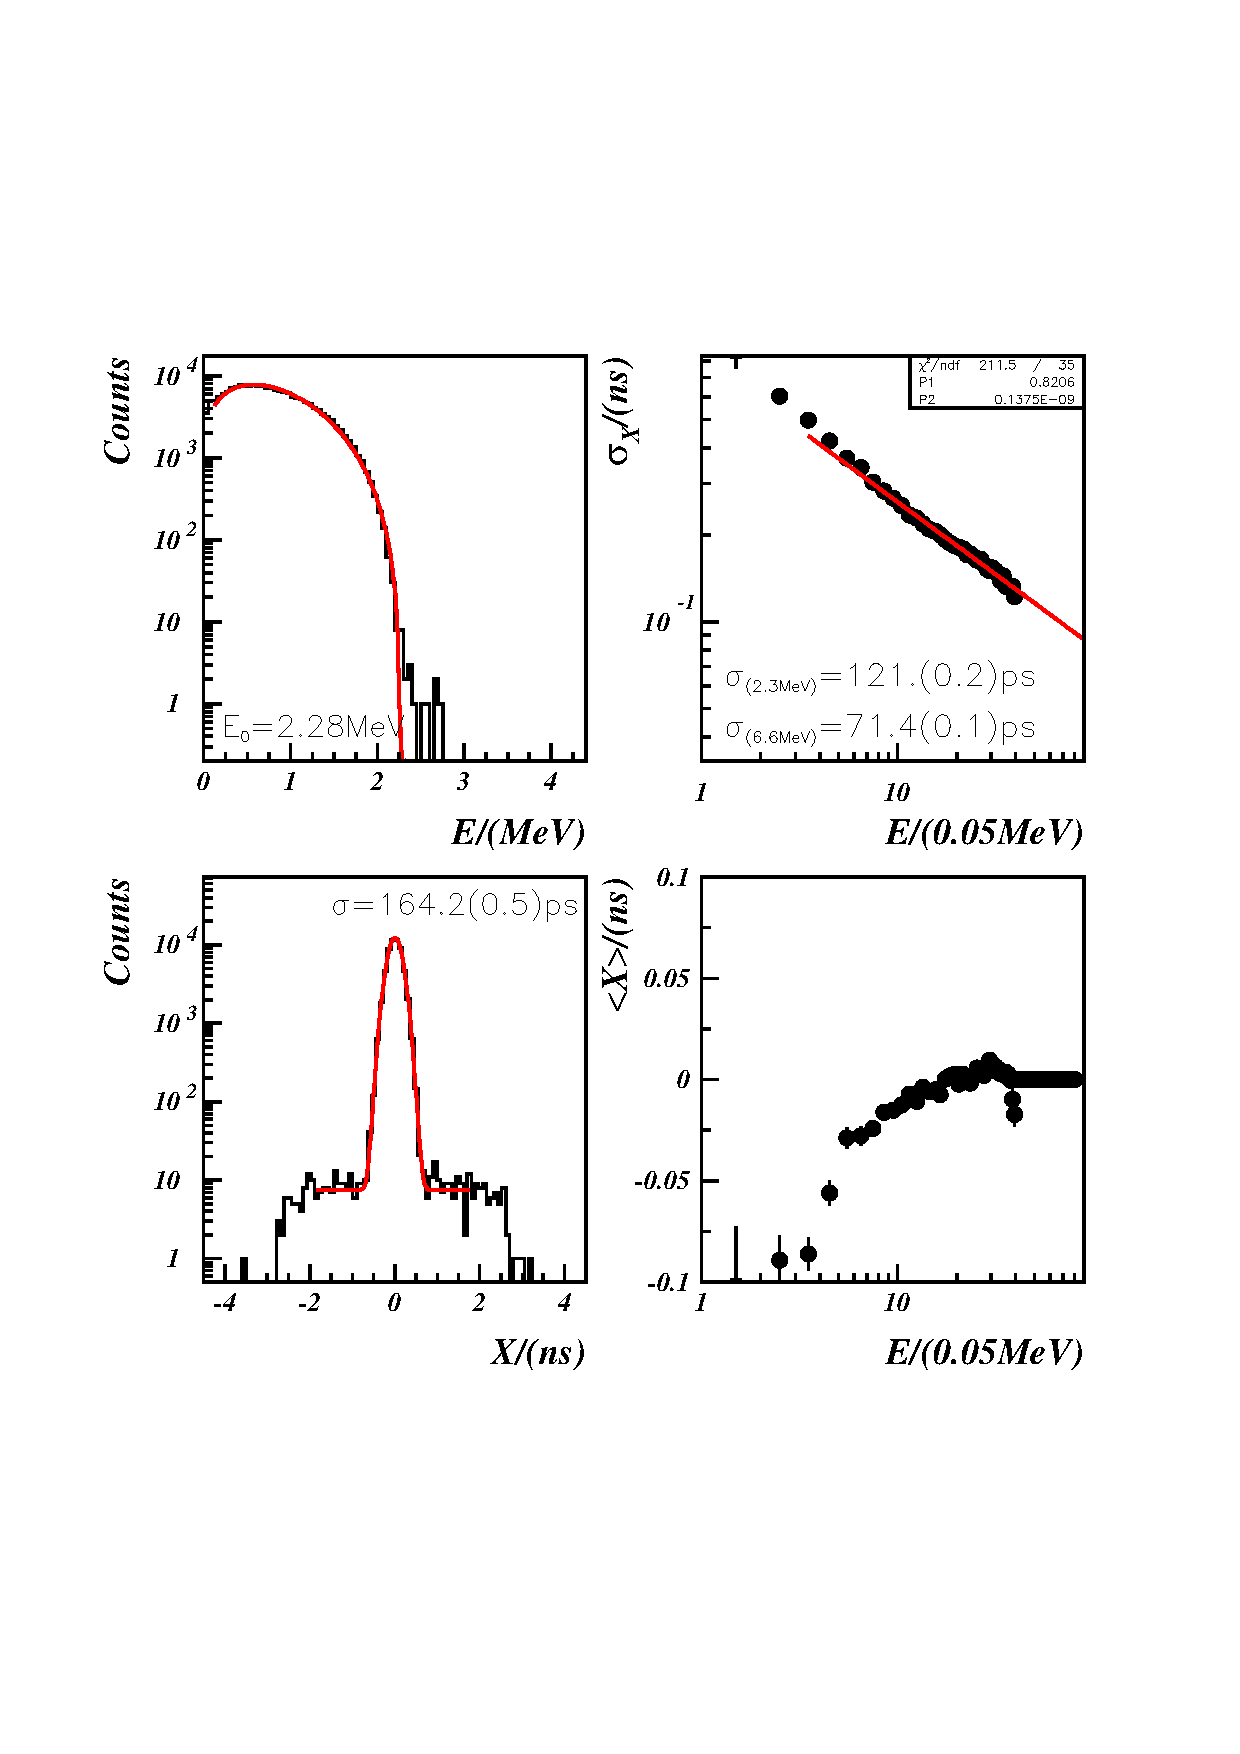
\includegraphics[width=13.8cm,clip=true,bb=20 150 620  720]{esxm_picture13.ps.gz}
\end{center}
\caption{
Effective time resolution of MCP PM Burle-85011   
obtained with the location method  of the 
 radiative source $^{90}Sr$   placed  in the center of the   counter.
Panel 
1)top-left: energy ($E$) spectrum of $\beta$-particles ;
2)bottom-left: coordinate distribution ($X$) of $\beta$-particles  with $E>1~MeV$; 
3)top-right: $\sigma_{X}$ of the peak vs $E$; 
4)bottom-right: $<X>$ vs  $E$.
\label{mcp85011sample}}
\end{figure}
\clearpage


\begin{figure}[htbp]%#32
\begin{center}
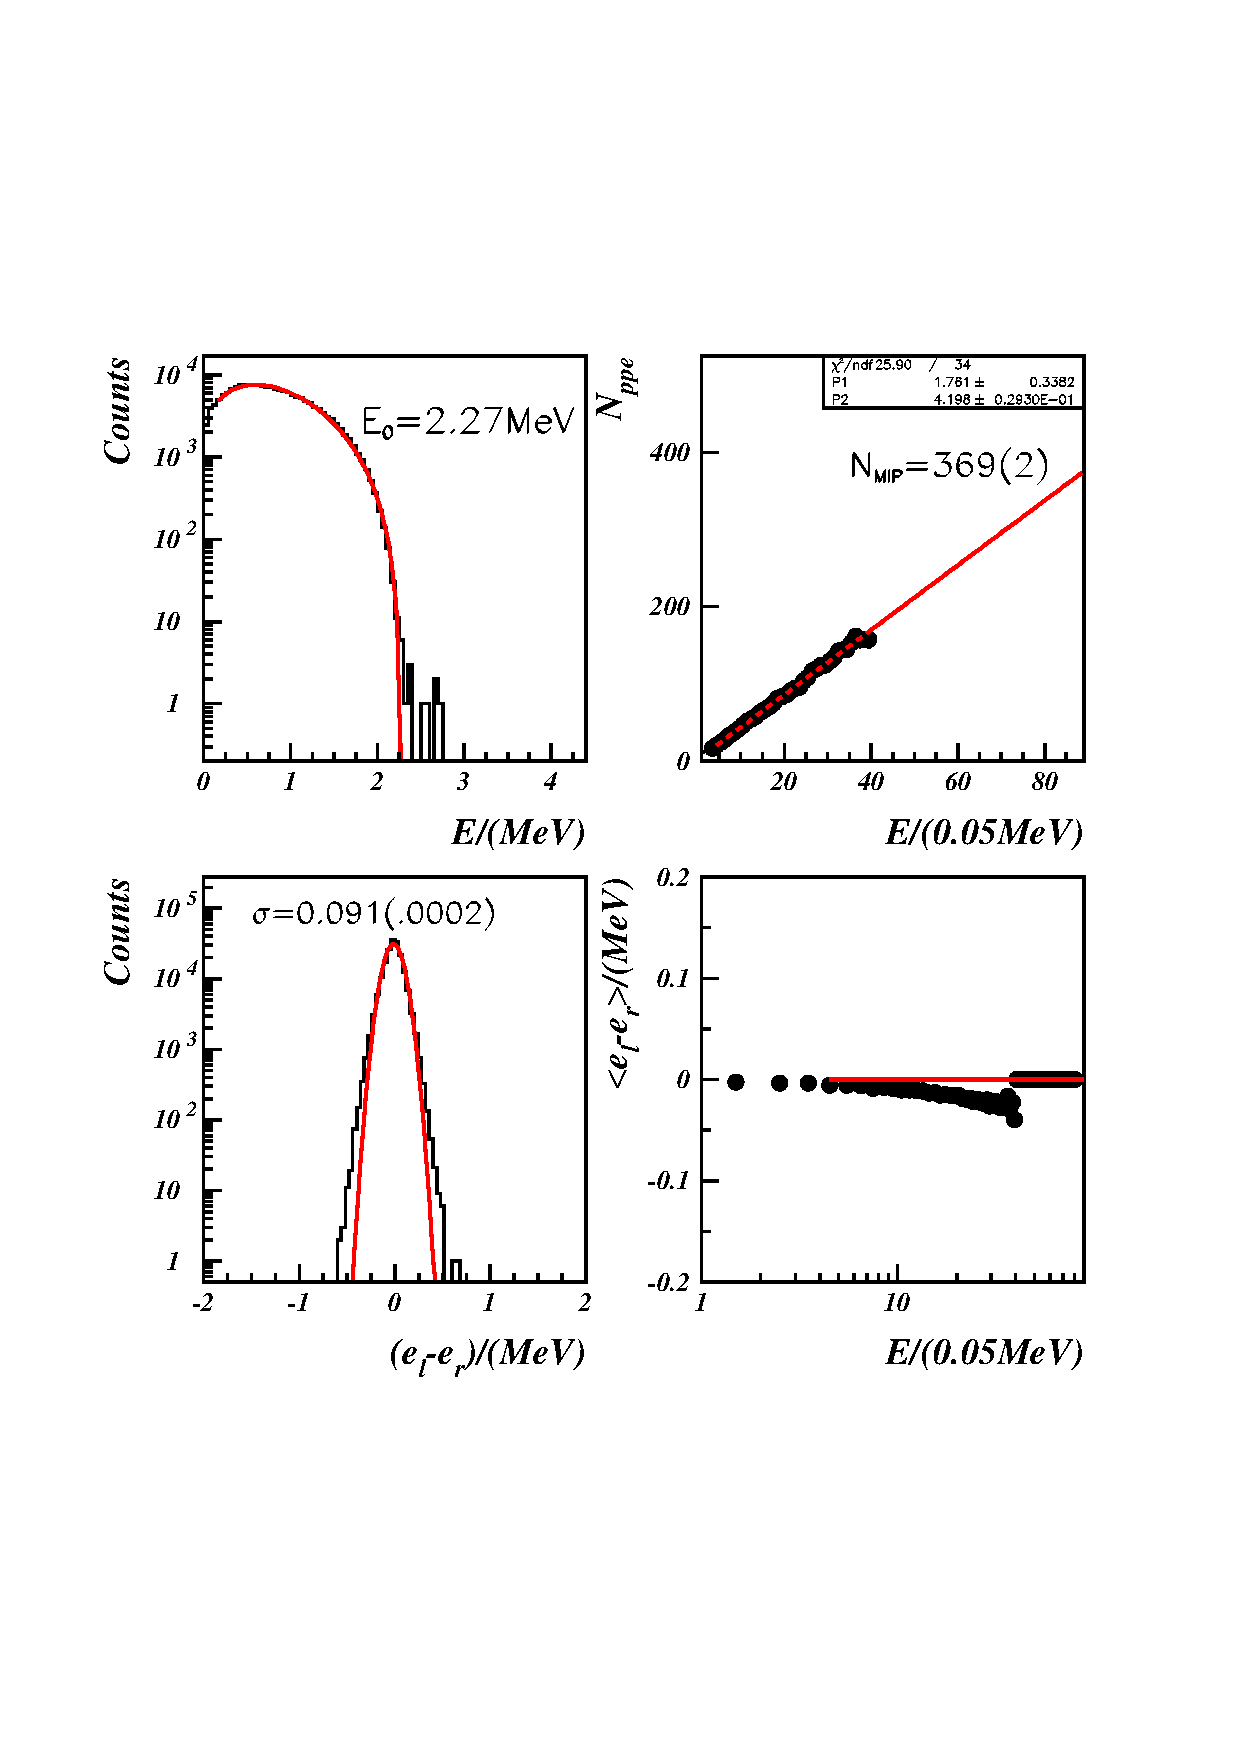
\includegraphics[width=13.8cm,clip=true,bb=20 150 620  720]{enppe_picture13.ps.gz}
\end{center}
\caption{Number of primary photoelectrons in Burle~85011.
1)Top-left: energy ($E$) spectrum of $\beta$-particles;
2)top-right:  $N_{ppe}$ vs $E$. It is expected to be $369\pm2$ at MIPs energy  $\approx4.4~MeV$;
3)bottom-left: spectrum of $(e_l-e_r)$, where $e_{l,r}$ are the energies measured from two sides of the counter;
4)bottom-right: mean value of $(e_l-e_r)$ vs  $\beta$-particle energy
\label{mcpnppe85011}}
\end{figure}
\clearpage


\begin{figure}[htbp]%#33
\begin{center}
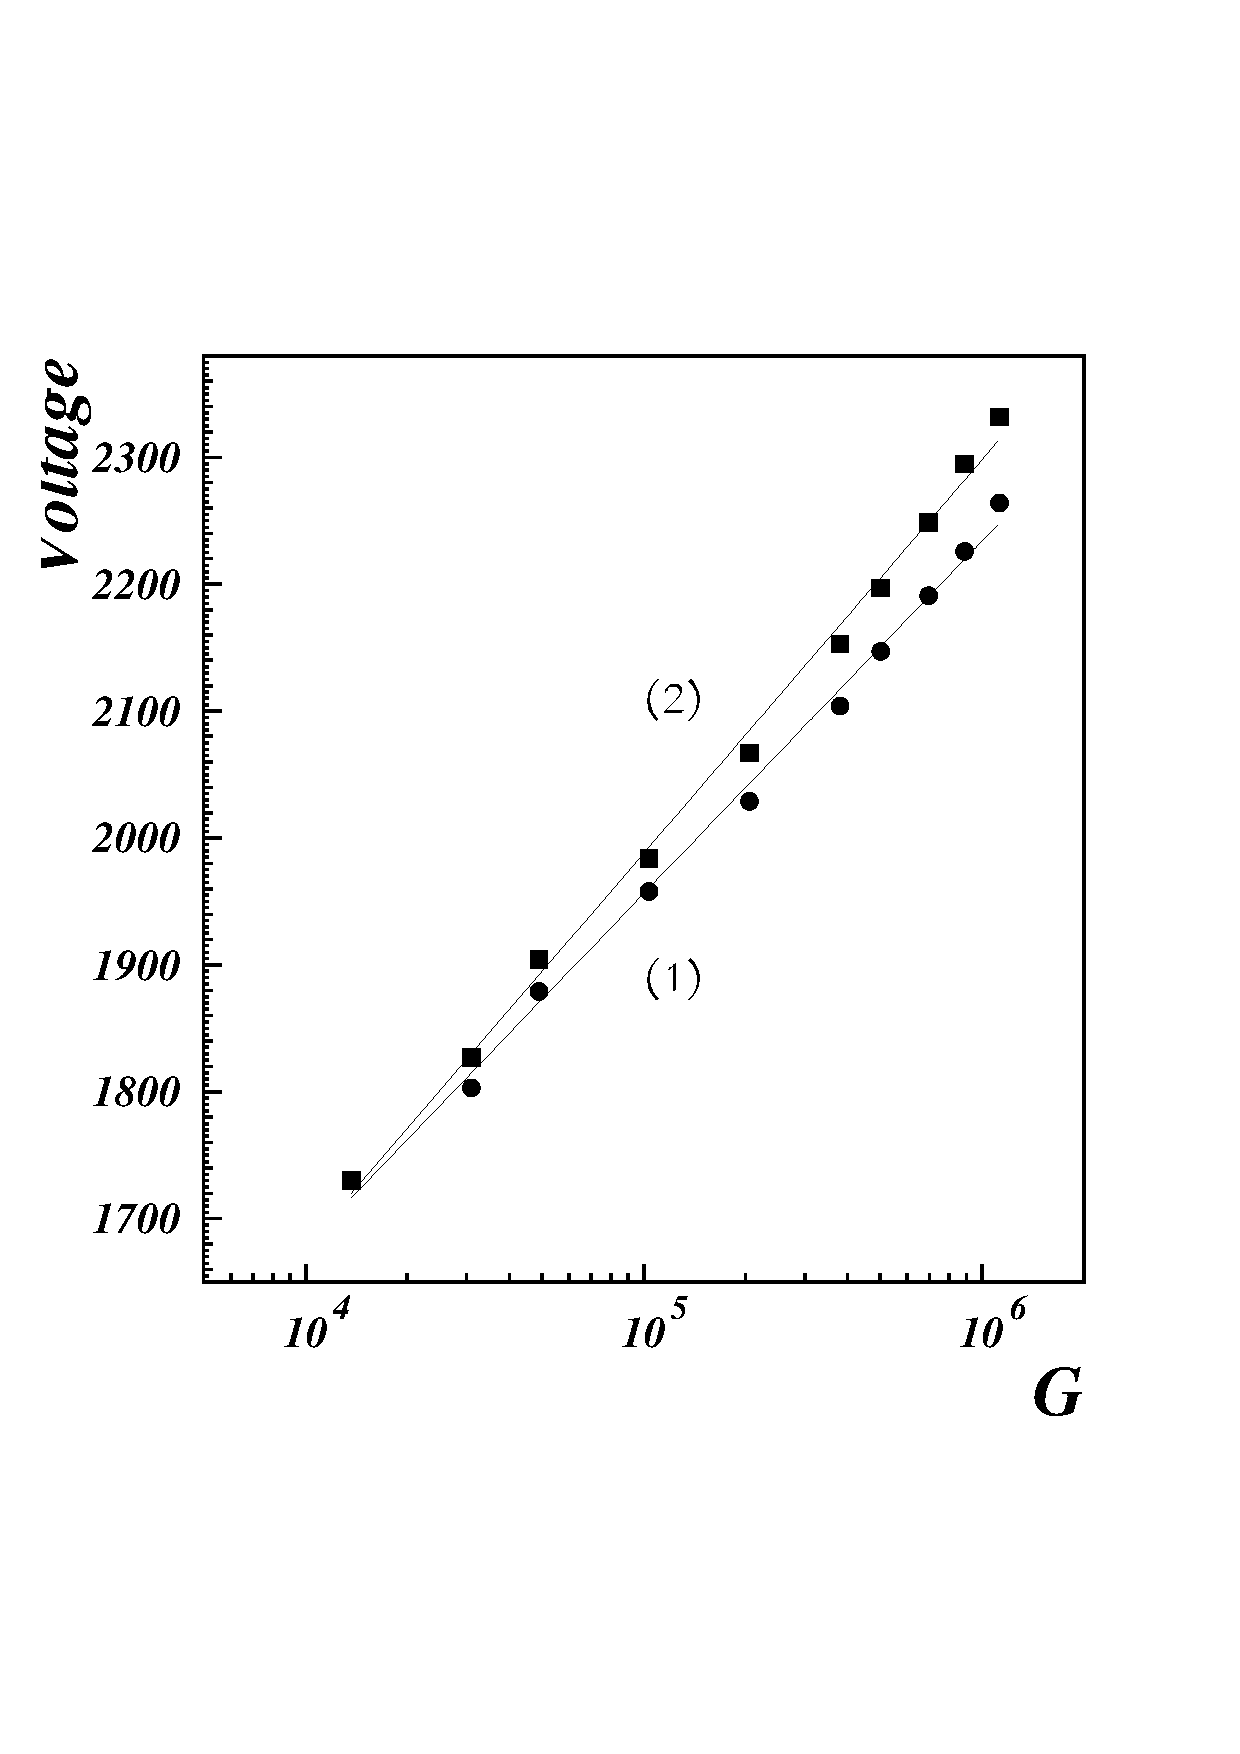
\includegraphics[height=13.8cm,clip=true,bb=20 150 620  720]{hvvsgain_picture85011.ps.gz}
\end{center}
\caption{High Voltage  vs Burle~85011 Gain.
The curves (1) and (2) are fits to the power law.
(1)-left  PM,(2)-right  PM.}
\label{hvvsgain85011}
\end{figure}
\clearpage

\begin{figure}[htbp]%#34
\begin{center}
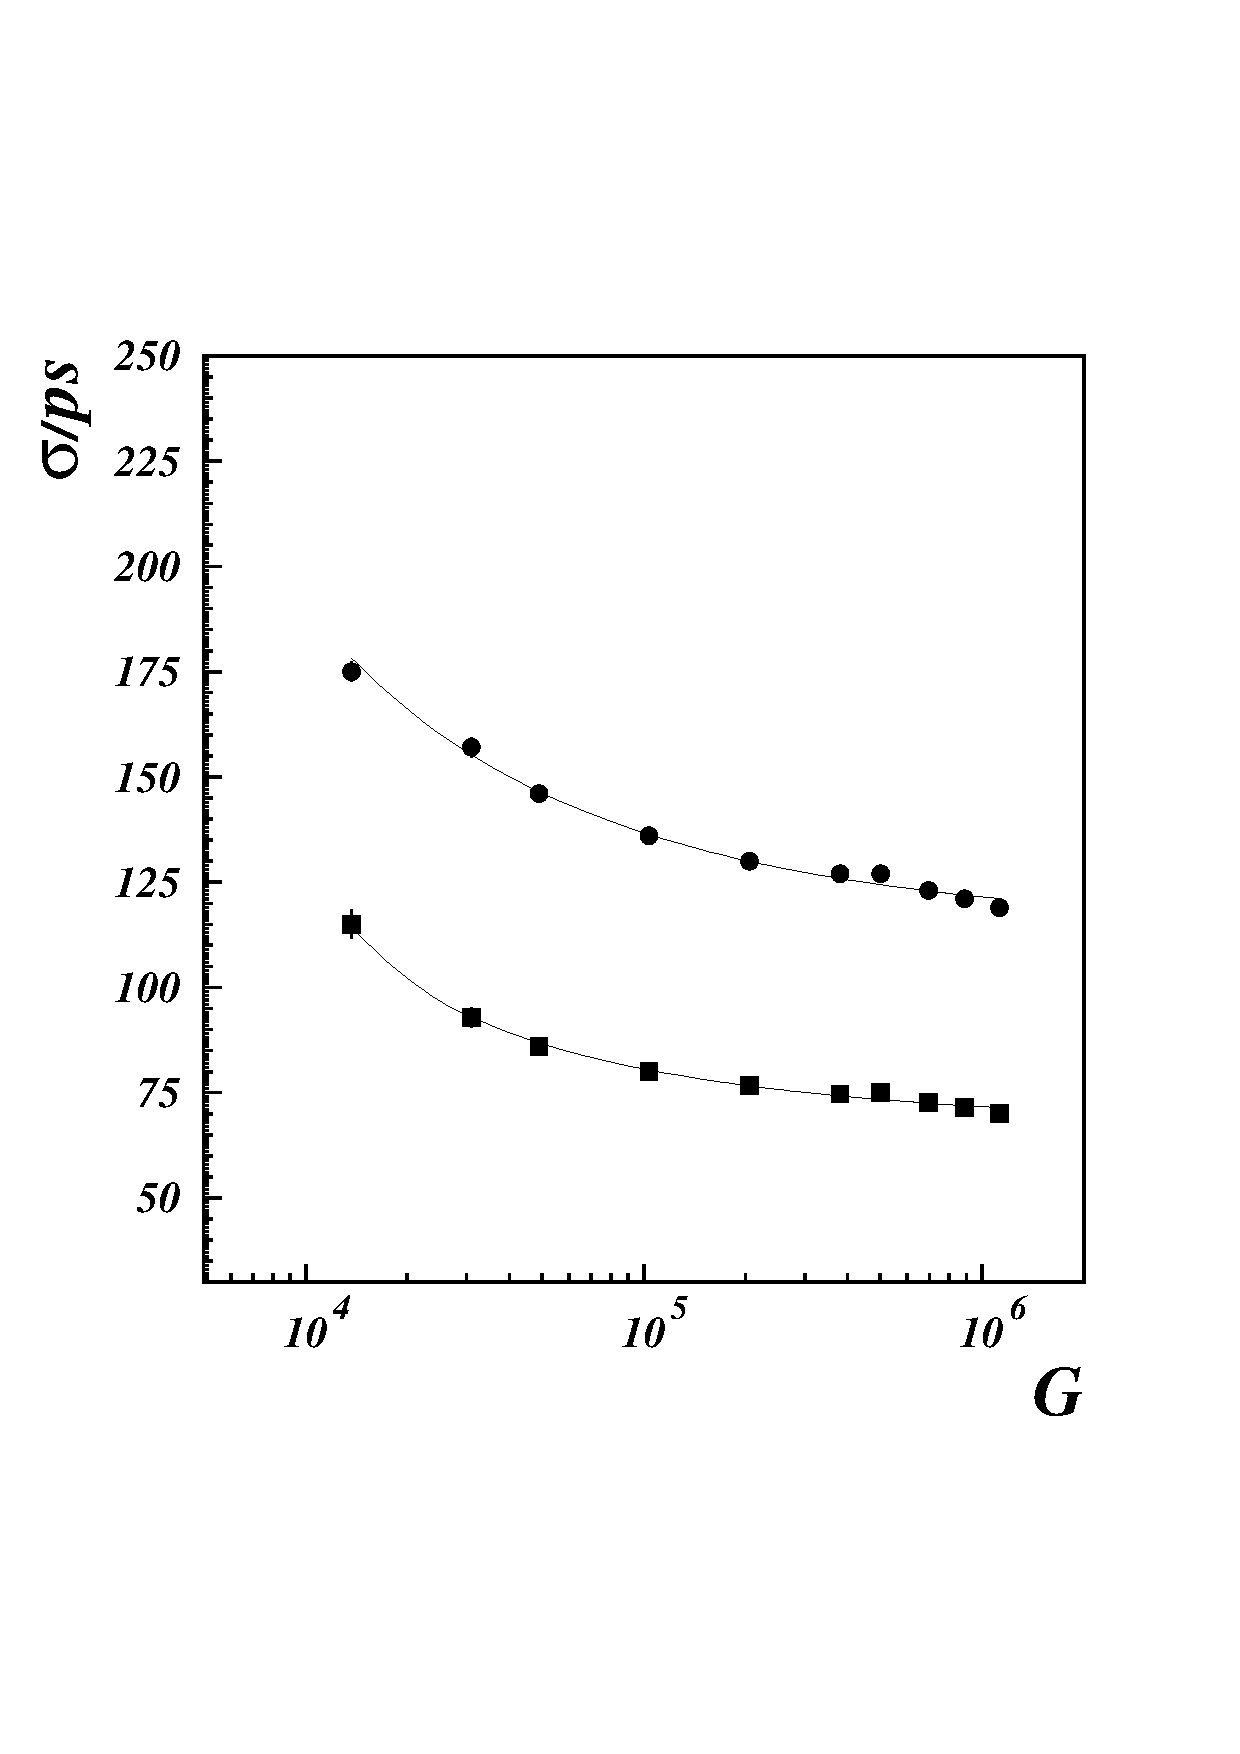
\includegraphics[height=13.8cm,clip=true,bb=20 150 620  720]{res85011vsgain_picture85011.ps.gz}
\end{center}
\caption{Resolution  of Burle~85011  vs gain(G). 
Circles are for the $\sigma$ at ${\Delta}E=2.28MeV$.
Squares are for extrapolation to  ${\Delta}E=6.6MeV$~(corresponds to MIPs in $3~cm$ thick scintillator).
The curves are  fits to the $G^{-2}$ dependence.  
Amplification factor to the PM signals is 50.}
\label{sigmamip85011}
\end{figure}

\clearpage

%\caption{Spectra of residual  measured with 
%%         two R7761-70 and four R2083 PMTS(right) and six R2083 PMTs.
%%         \label{fig:res}}
%\end{figure}
%%%%%%%%%%%%%%%%%%%%%%%%%%%%%%%%%%%%%%%%%%%%
%%\begin{figure}[htbp]%#35
%%\begin{center}
%%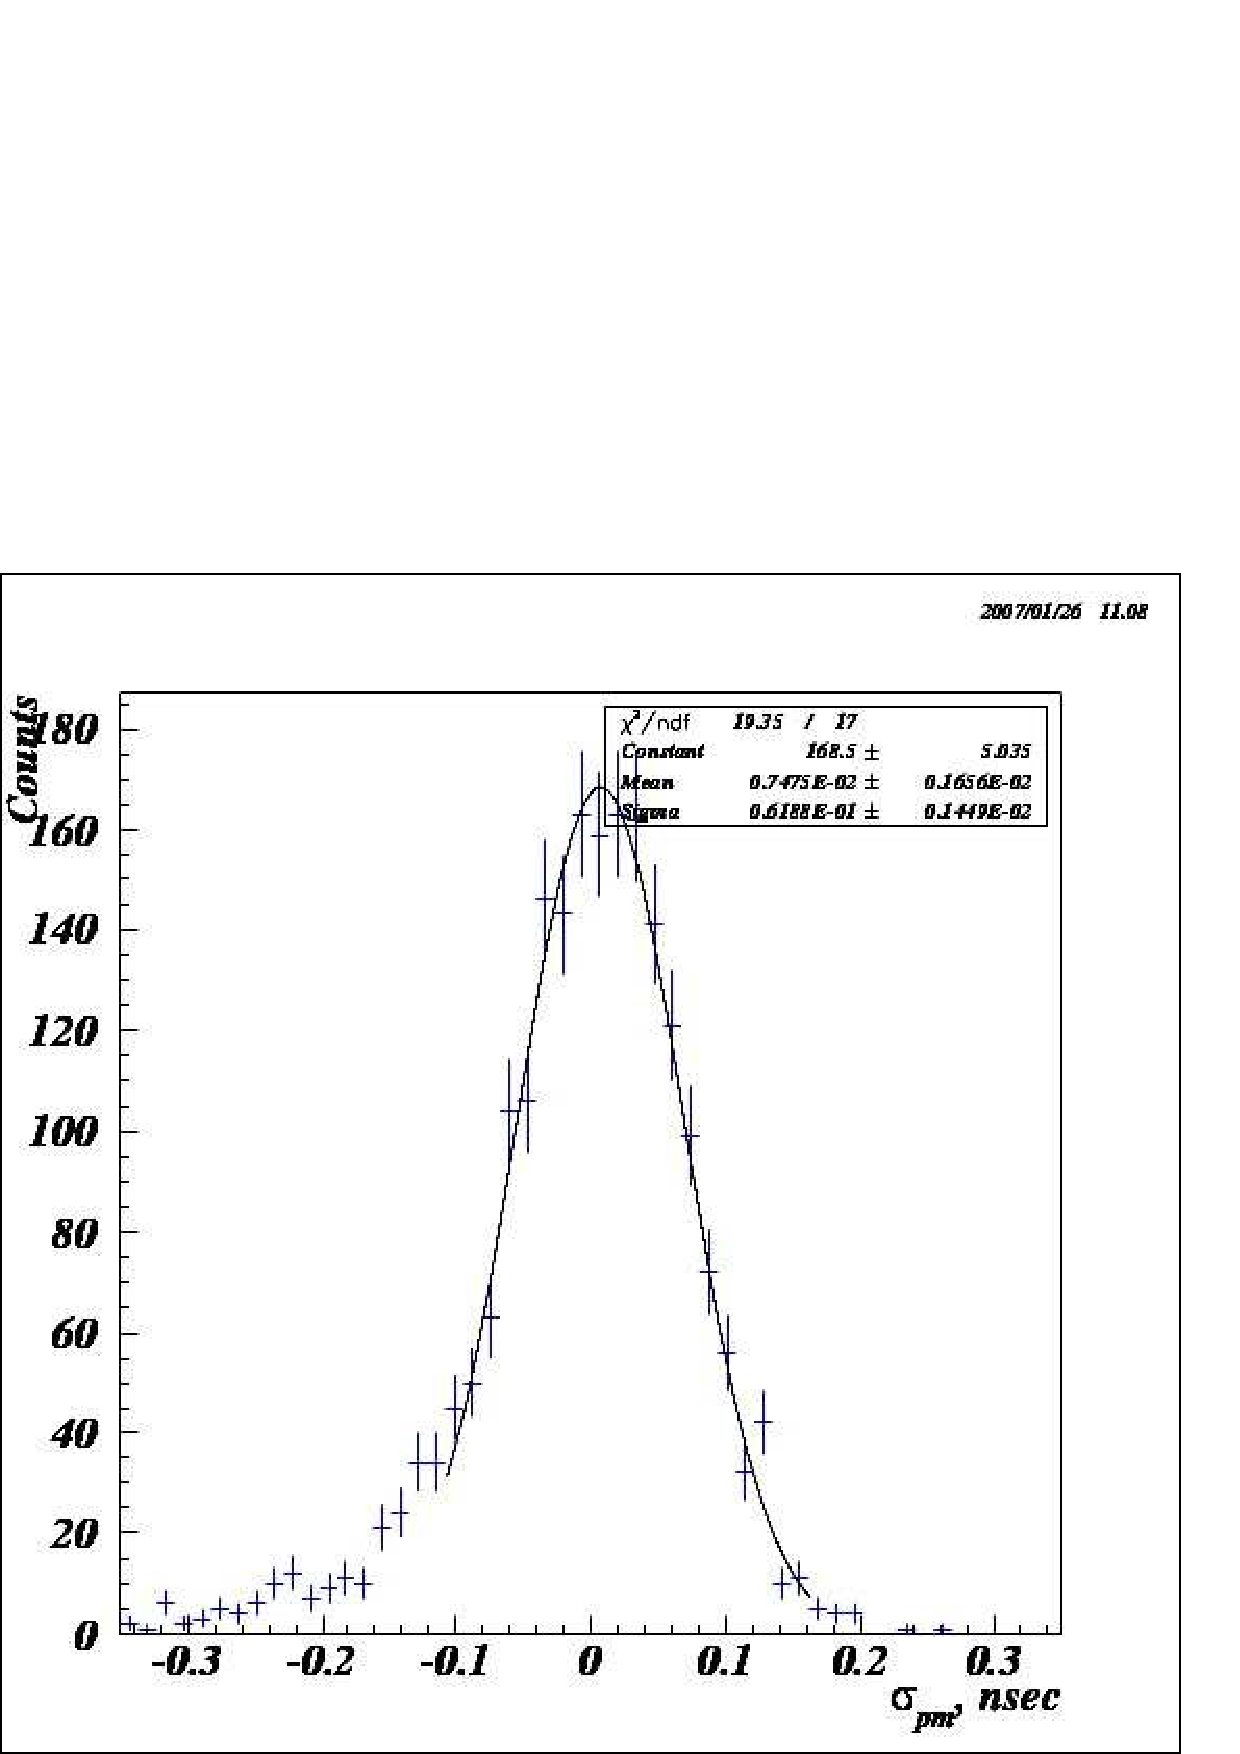
\includegraphics[height=13.8cm,clip=true,bb=20 0 620  720]{res5505.ps.gz}
%%\end{center}

%%%%%%%%%%%%%%%%%FIG.2%%%%%%%%%%%%%%%%%%%%%%
\begin{figure}[ht]
\vspace*{0.2cm}
\epsfverbosetrue\epsfxsize=6.5cm\epsfysize=7cm\epsfbox{tau041007.eps}
\hspace*{0.4cm}\epsfverbosetrue\epsfxsize=6.5cm\epsfysize=7cm\epsfbox{tau0117a.eps}
\vspace*{-0.3cm}
\caption{Spectra of 6 PMT time residuals scaled by $\frac{2}{\sqrt{3}}$.
 Left panel: distribution  with two R7761-70 and four R2083 PMTS(right).  
Right panel: distribution obtained with with  six R2083 PMTs.
The actual effective  $\sigma_{R7761}=64~ps$ yields from the $rms$ of the  left  panel.
The  reference  $\sigma_{R2083}=52\pm1ps$ at the right  panel  
coincides with the previously reported value from Table~\ref{crt}.
\label{finemesh01}}
\end{figure}
\clearpage

\begin{figure}[htbp]%#4
\begin{center}
%\includegraphics[width=13.8cm,clip=true,bb=-0 -40 720  800]{/home/prof/batourine/knu/publications/rep_llg_fromJLAB/cosmic-6pmtllg_picture.ps.gz}
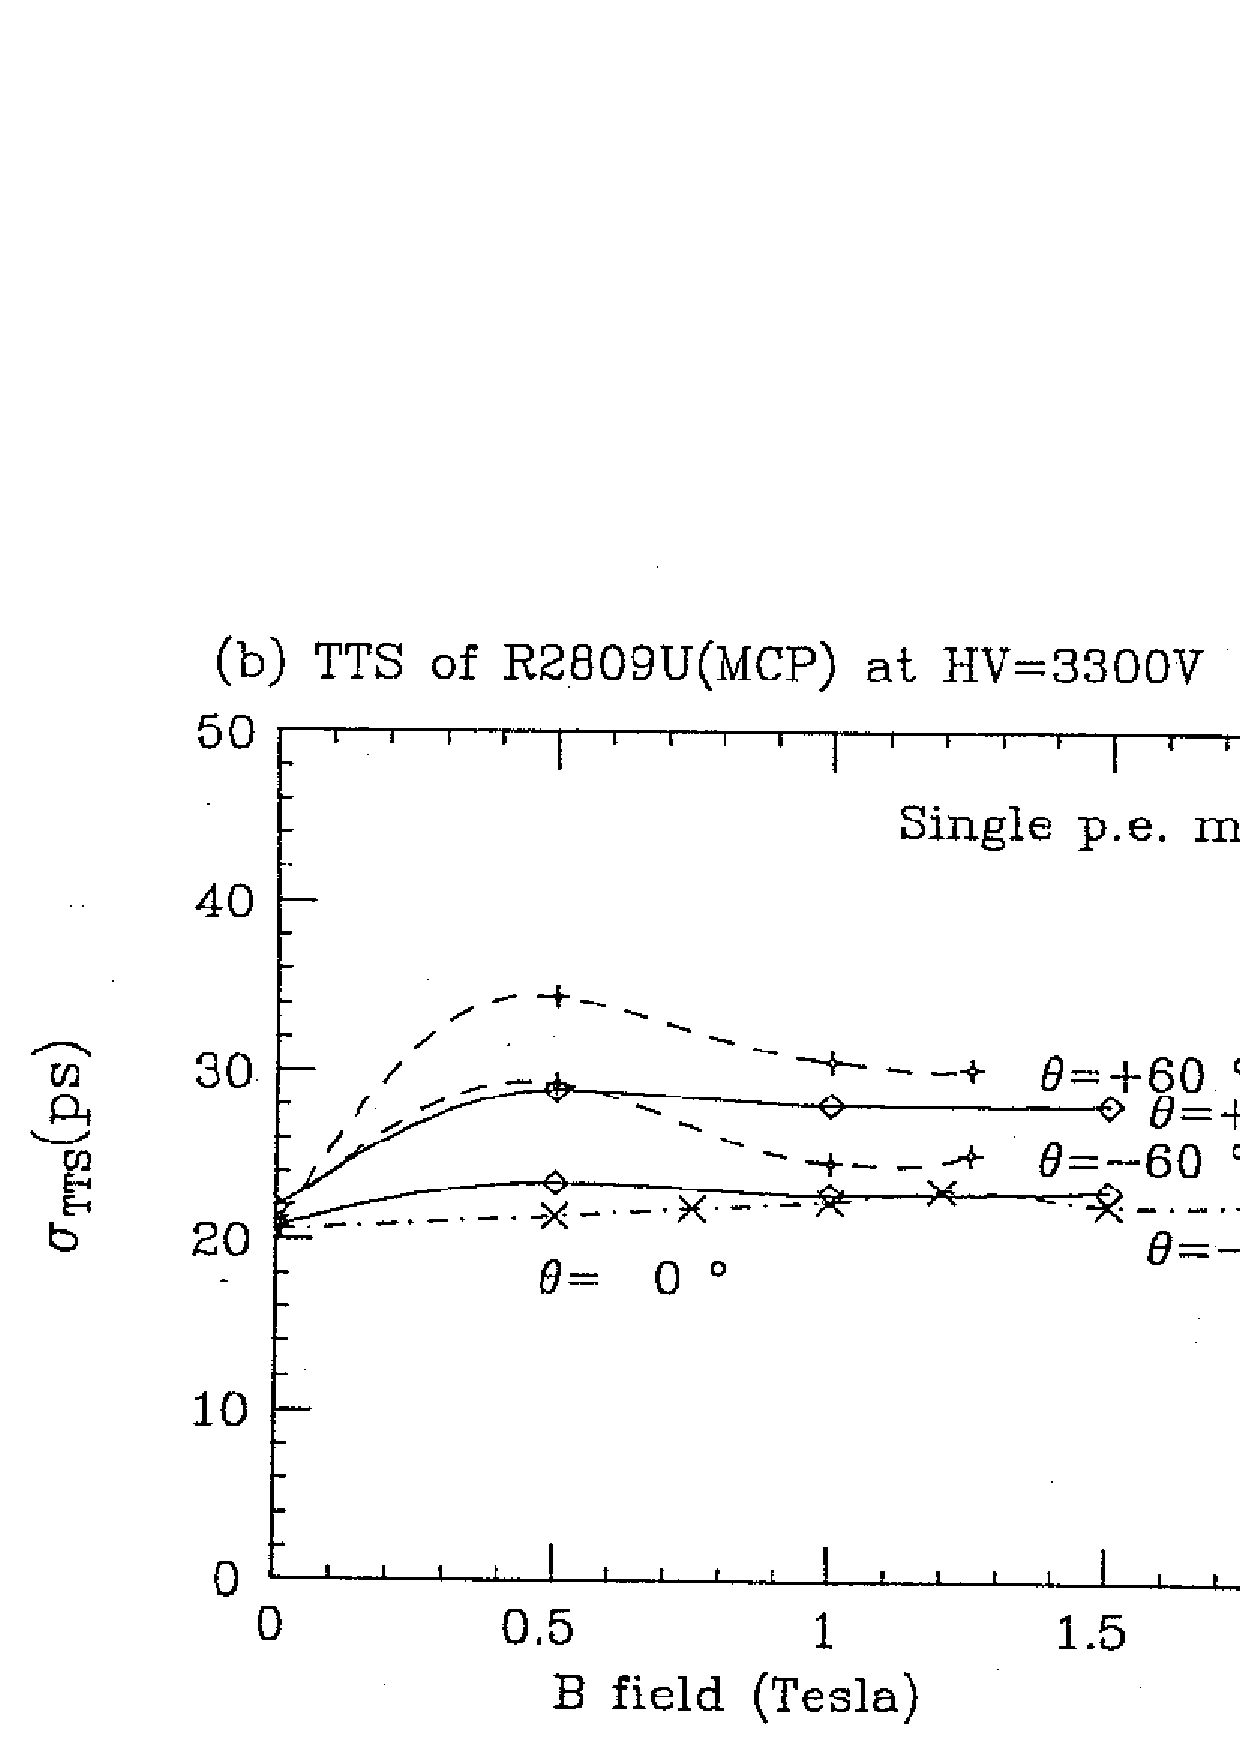
\includegraphics[width=13.8cm,clip=true,bb=20 150 620  720]{fig02MC.ps.gz}
\end{center}
\caption{%fig02MC.ps.gz,
Transition Time Spread of the MCP PM  vs magnetic field.
\label{mcpt}}
\end{figure}
\clearpage

\begin{figure}[htbp]%#5
\begin{center}
%\includegraphics[width=13.8cm,clip=true,bb=-0 -40 720  800]{/home/prof/batourine/knu/publications/rep_llg_fromJLAB/cosmic-6pmtllg_picture.ps.gz}
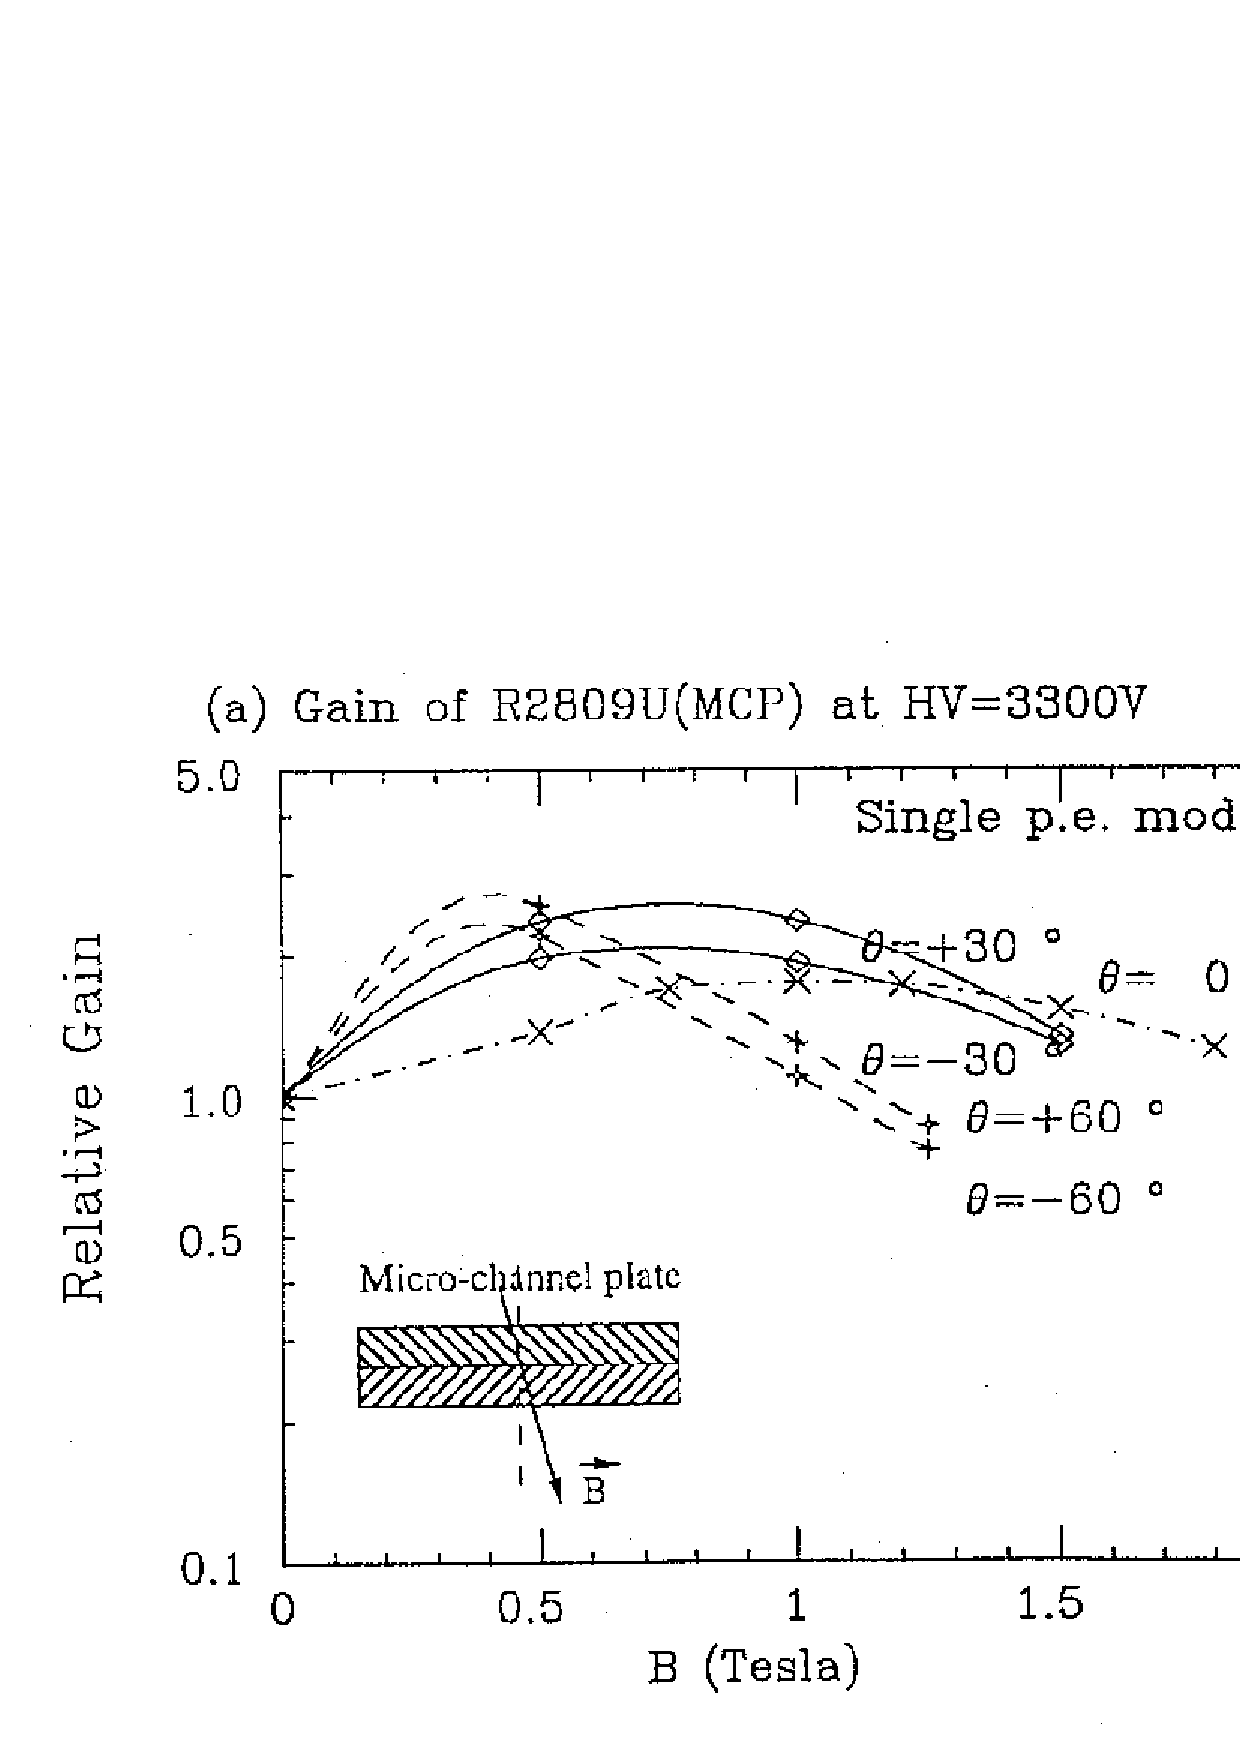
\includegraphics[width=13.8cm,clip=true,bb=20 150 620  720]{fig01MC.ps.gz}
\end{center}
\caption{%fig01MC.ps.gz,
Gain of the MCP PM  vs magnetic field at different orientations. 
\label{mcpg}}
\end{figure}
\clearpage



\begin{figure}[htbp]%#6
\begin{center}
%\includegraphics[width=13.8cm,clip=true,bb=-0 -40 720  800]{/home/prof/batourine/knu/publications/rep_llg_fromJLAB/cosmic-6pmtllg_picture.ps.gz}
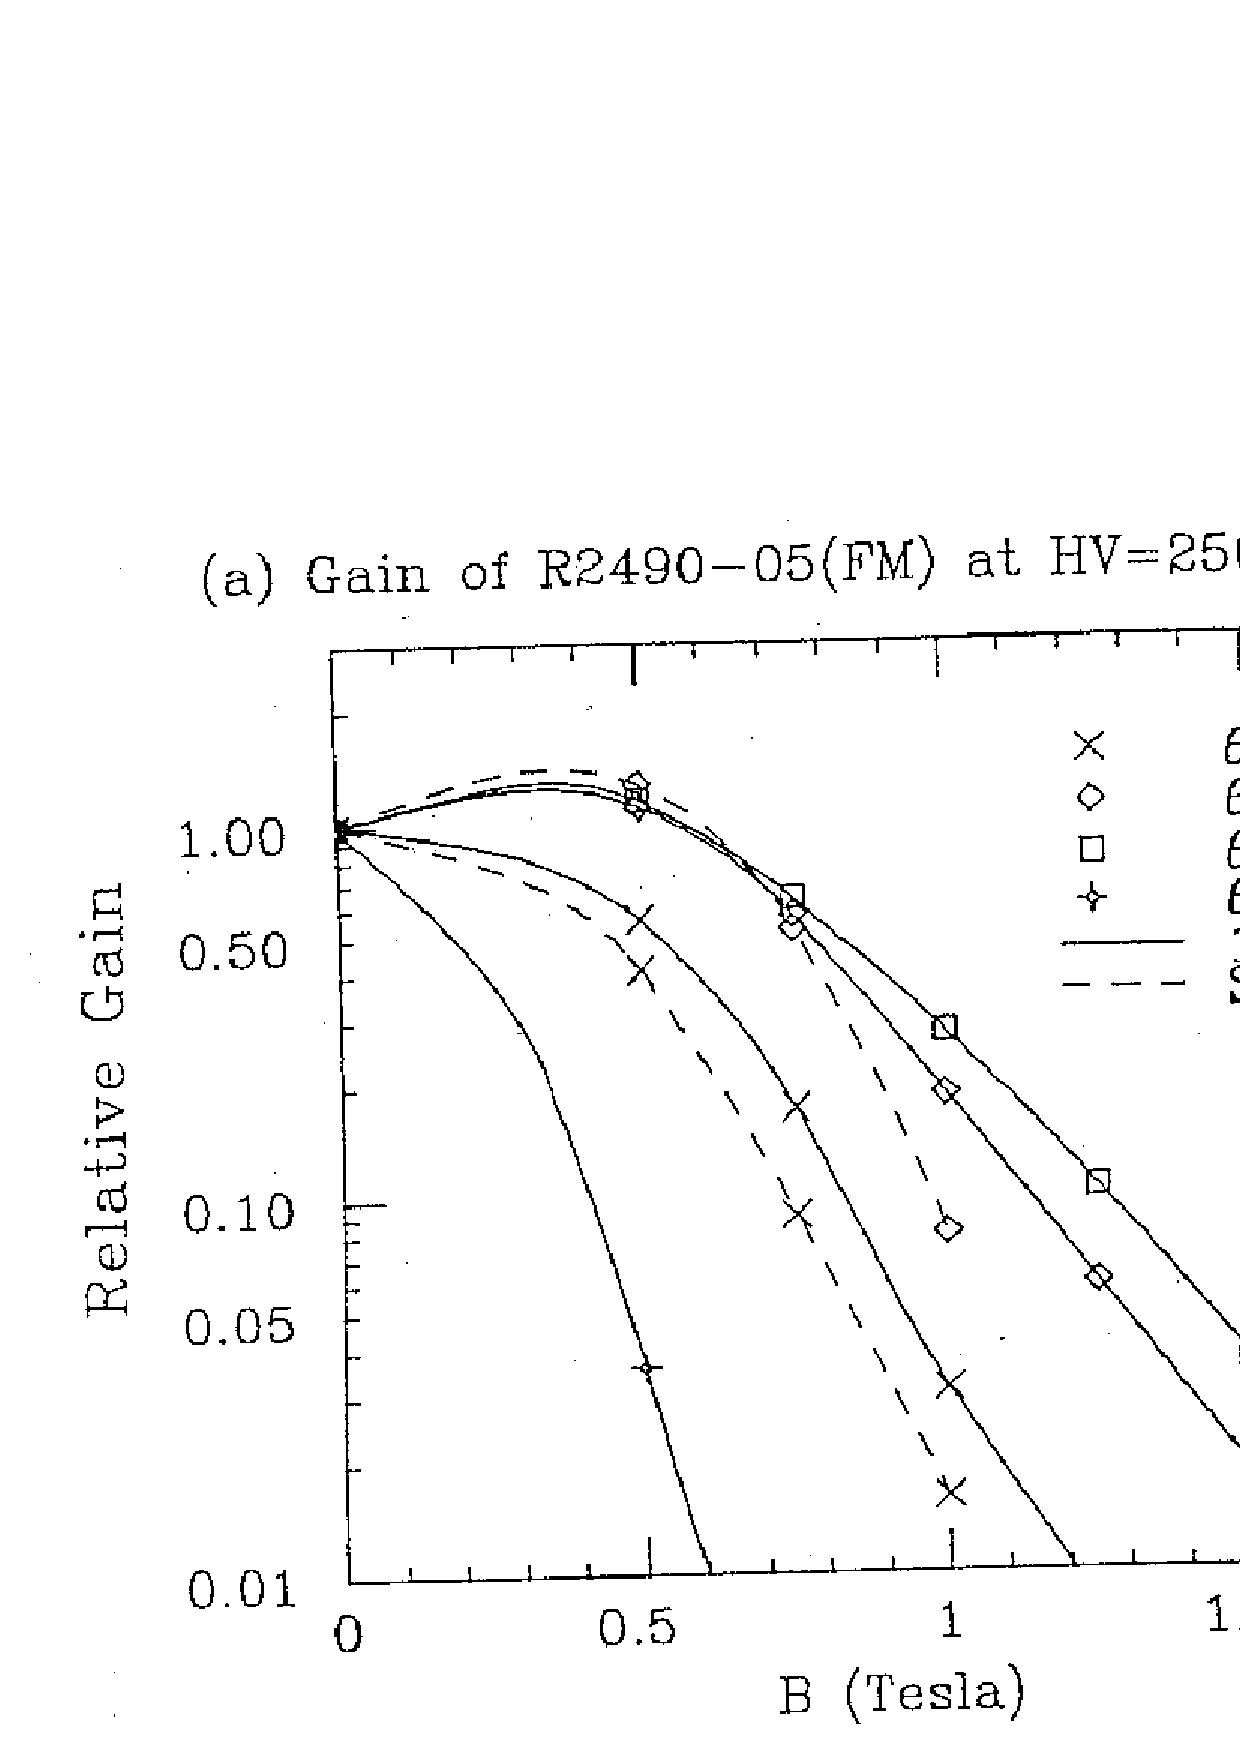
\includegraphics[width=13.8cm,clip=true,bb=20 150 620  720]{fig03MC.ps.gz}
\end{center}
\caption{%fig03MC.ps.gz,
Gain of the fine mesh PM R2490-05 vs magnetic field at different orientations. 
\label{fmg}}
\end{figure}
\clearpage


\begin{figure}[htbp]%#7
\begin{center}
%\includegraphics[width=13.8cm,clip=true,bb=-0 -40 720  800]{/home/prof/batourine/knu/publications/rep_llg_fromJLAB/cosmic-6pmtllg_picture.ps.gz}
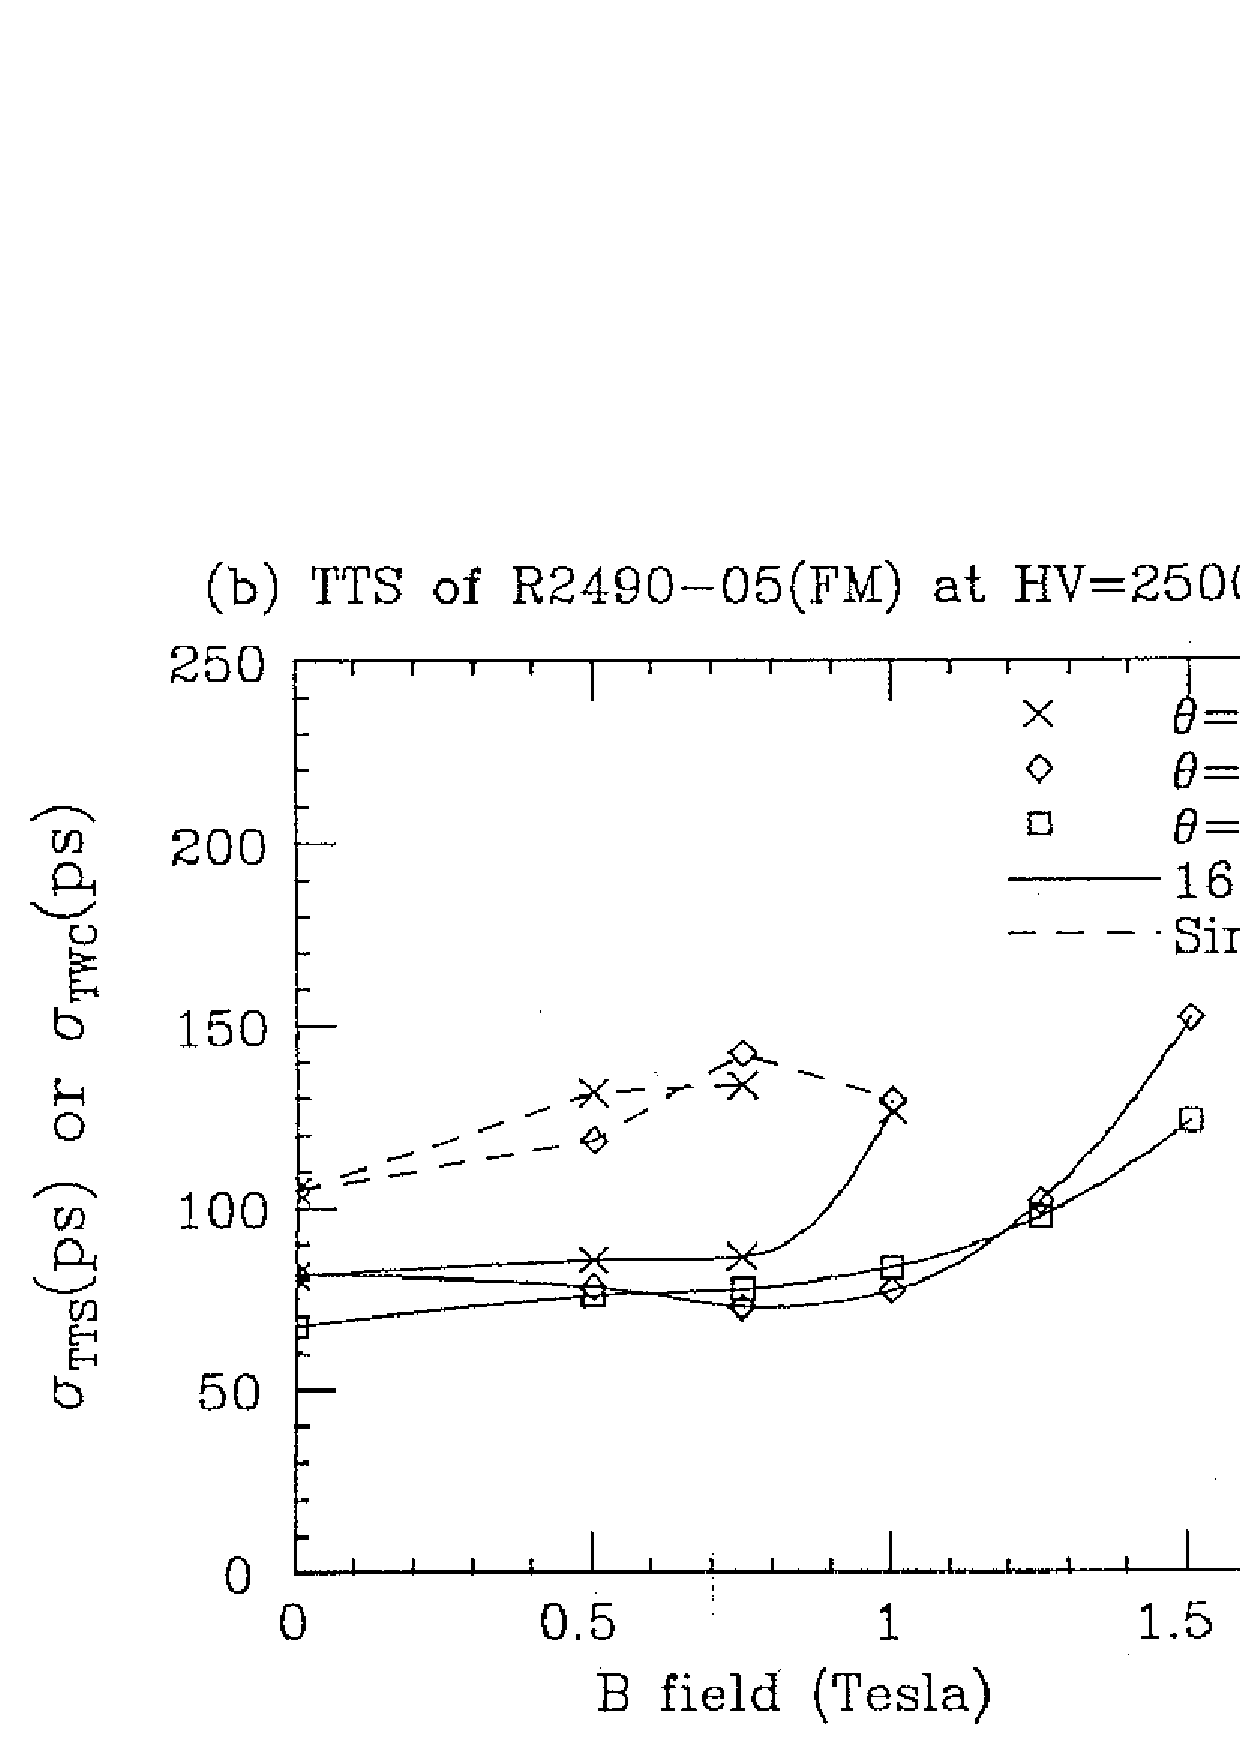
\includegraphics[width=13.8cm,clip=true,bb=20 150 620  720]{fig04MC.ps.gz}
\end{center}
\caption{%fig04MC.ps.gz,
Transition Time Spread of the fine mesh PM R2490-05 vs magnetic field.
\label{fmt}}
\end{figure}
\clearpage


\begin{figure}[htbp]%#8
\begin{center}
%\includegraphics[width=14cm,clip=true,bb=80 0 550  800]{/home/prof/batourine/fig/bentlg03.ps.gz}
%\includegraphics[width=14cm,clip=true,bb=55 0 550  750]{./bentlg03.ps.gz}
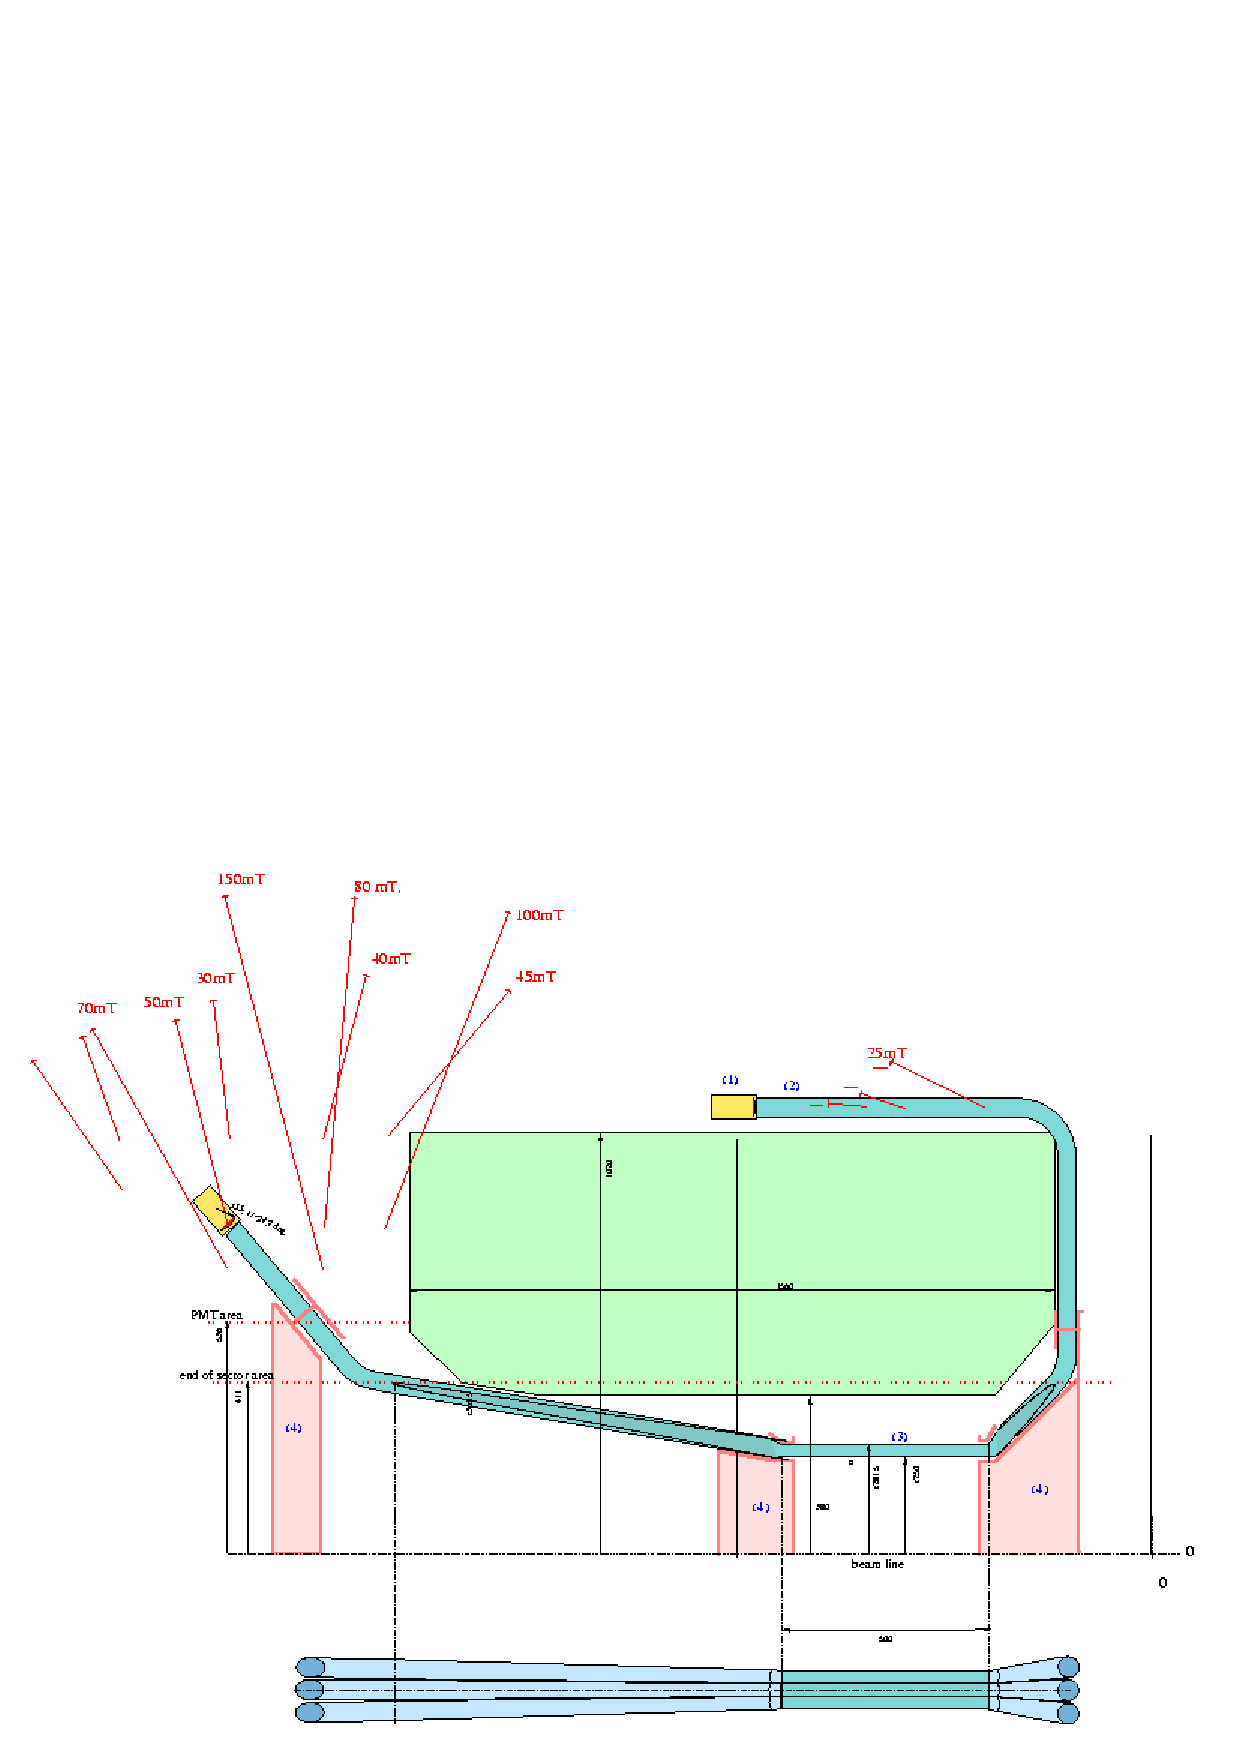
\includegraphics[width=22cm,clip=true,bb=100 40 750 590]{JLABt0R2083-2.ps.gz}
\end{center}
\caption{%JLABt0R2083-2.ps.gz
The pilot design  of the CLAS12 CTOF counter.
 (1)-PMT R2083 from Hamamatsu, (2)- acrylic light guides,
(4)-supporting cones and rings, (3)-scintillators.
Magnetic field is shown by vectors.
\label{bentlg03}}
\end{figure}
%\addtocontents{lof}{List of figures}
\clearpage


\newpage
\begin{figure}[htbp]%[h]#9
\begin{center}
%\includegraphics[height=17cm,clip=true,bb=100 0 500  760]{/home/prof/batourine/fig/bentlgupdownstream.ps.gz}
\includegraphics[height=17cm,clip=true,bb=100 0 500  760]{bentlgupdownstream.ps.gz}
\end{center}
\caption{%bentlgupdownstream.ps.gz,
Upstream (1) and downstream (2) view of the CTOF detector.
\label{bentlgud03}}
\end{figure}
\clearpage

%
\newpage
\begin{figure}[htbp]%#10
\begin{center}
%\includegraphics[height=14cm,clip=true,bb=75 100 555  680]{/home/prof/batourine/fig/t0sccross.ps.gz}
\includegraphics[height=14cm,clip=true,bb=75 100 555  680]{t0sccross.ps.gz}
\end{center}
\caption{%t0sccross.ps.gz,
The cross section of the scintillator inscribed into the 
photo-cathode of R2083 from Hamamatsu.  
Light guides will  join PMTs via the
cylindrical side of the same diameter as
the  R2083 photo-cathode, i.e. $46~mm$. 
\label{sccross}}
\end{figure}
\clearpage


\newpage

\begin{figure}[htbp]%#11
\begin{center}
%\includegraphics[width=13.8cm,clip=true,bb=-0 -40 720  800]{/home/prof/batourine/knu/publications/rep_llg_fromJLAB/transitionvscyl.ps.gz}
\includegraphics[width=13.8cm,clip=true,bb=20 100 620  720]{transitionvscyl.ps.gz}
\end{center}
\caption{%transitionvscyl.ps.gz,
The light transportation efficiency(vertical scale)  of the ``pyramid'' light guide vs the length 
(horizontal scale) of the milled surface.
\label{plgef}}
\end{figure}
\clearpage


\begin{figure}[htbp]%#12
\begin{center}
%\includegraphics[width=13.8cm,clip=true,bb=-0 80 700 800]{/home/prof/batourine/fig/t0lgupstr.ps.gz}
\includegraphics[width=13.8cm,clip=true,bb=-0 -40 600 800]{t0lgupstr.ps.gz}
\end{center}
\caption{%t0lgupstr.ps.gz,
The design of the upstream light guide.
\label{lgupstream}}
\end{figure}
\clearpage

%\newpage
%\begin{figure}[h]%#13
%\begin{center}
%\includegraphics[width=13.8cm,clip=true,bb=-0 -40 320  300]{./figures_llg/polishingLightGuide3.eps}
%\end{center}
%\caption{Manufacturing the $1m$-long light guides.}
%\label{lgmanu}
%\end{figure}

\clearpage
\newpage
\begin{figure}[htbp]%#13
\begin{center}
%\includegraphics[width=13.8cm,clip=true,bb=-0 -80 700 800]{/home/prof/batourine/fig/t0lgdown.ps.gz}
\includegraphics[width=13.8cm,clip=true,bb=-0 -40 600 800]{t0lgdown.ps.gz}
\end{center}
\caption{%t0lgdown.ps.gz,
The design of the downstream   $1m$-long light guide}
\label{lgdownstream}
\end{figure}
\clearpage


\begin{figure}[htbp]%#14
\begin{center}
%\includegraphics[width=13.8cm,clip=true,bb=-0 -40 720  800]{/home/prof/batourine/knu/publications/rep_llg_fromJLAB/transitionvscyl.ps.gz}
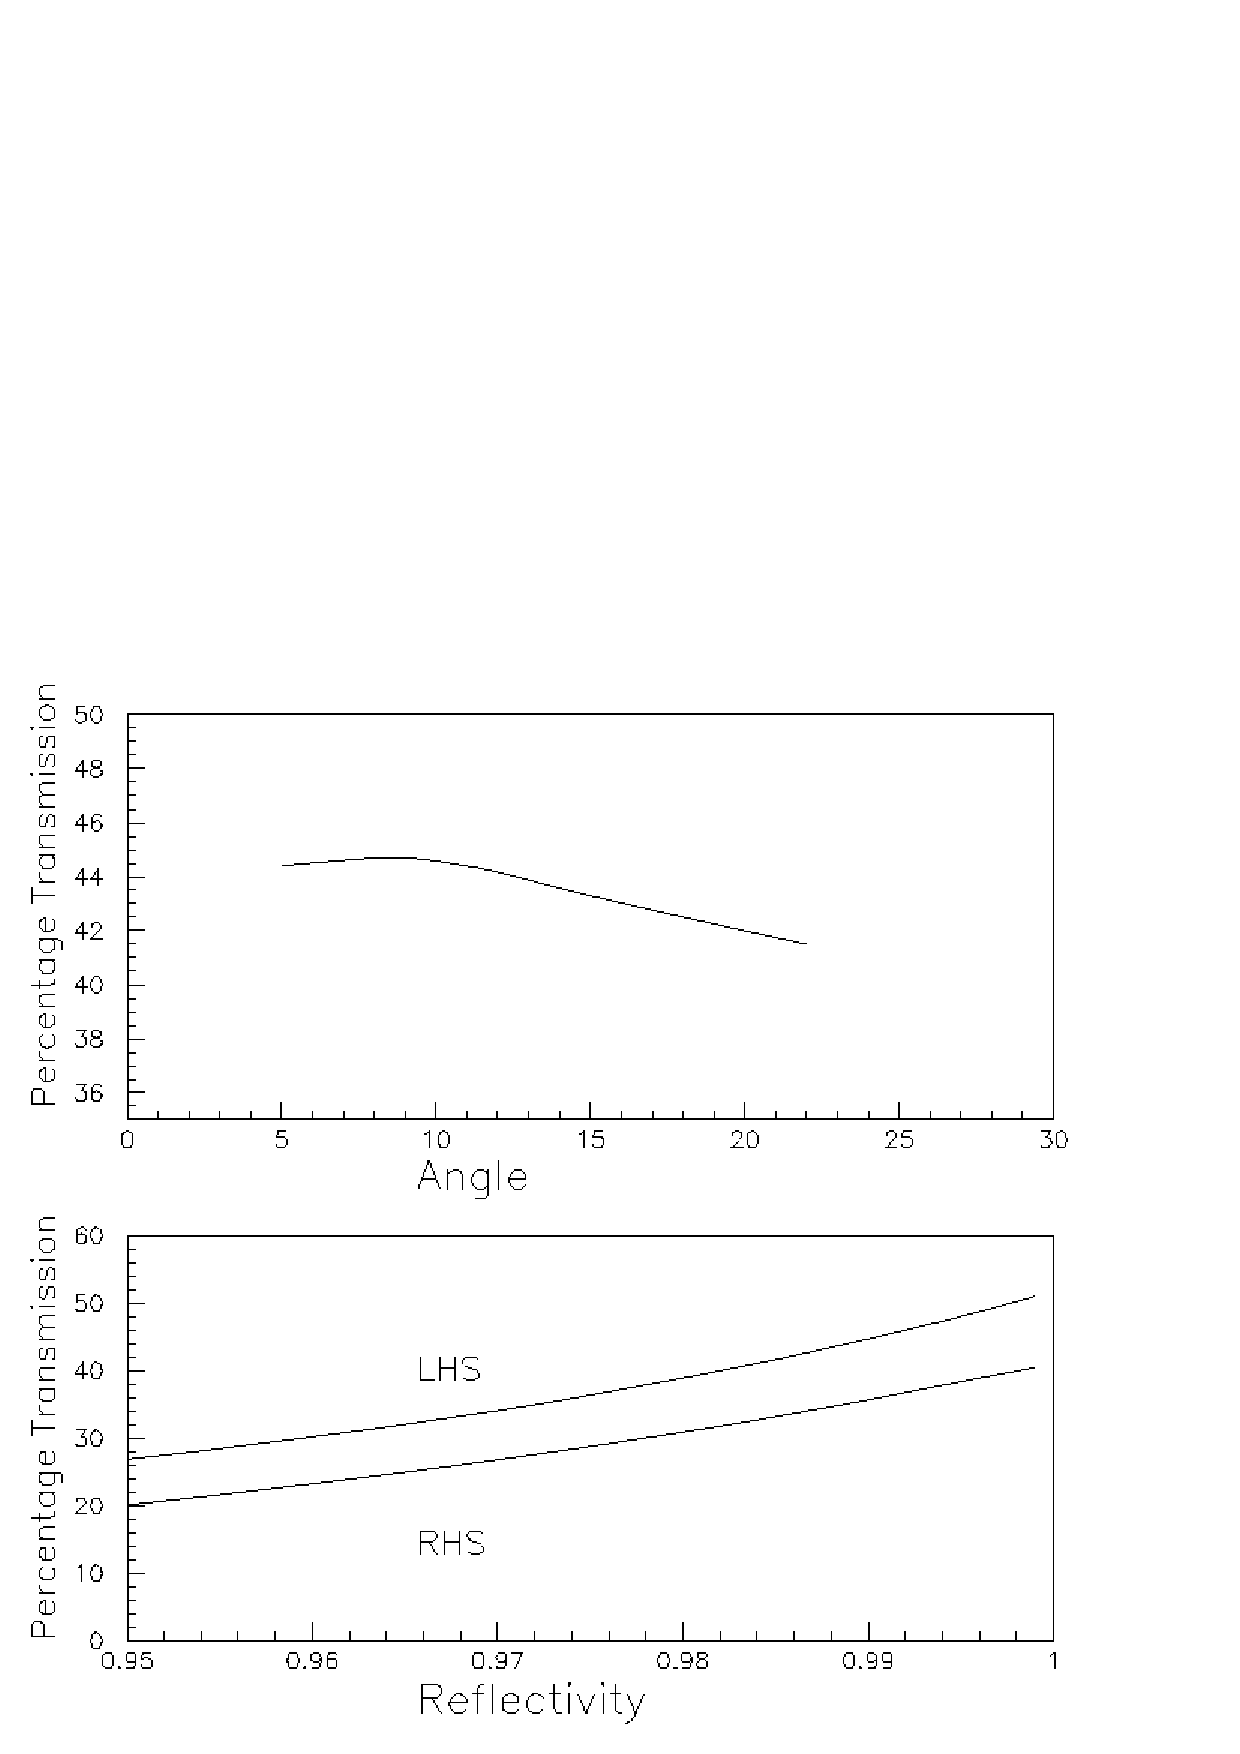
\includegraphics[width=13.8cm,clip=true,bb=20 100 620  720]{trans.ps.gz}
\end{center}
\caption{%trans.ps.gz,
Light transmission  vs 1) the ``down mirror'' orientation angle(left panel)
2) the reflectivity of the light guide surface(right panel).
\label{trans}}
\end{figure}
\clearpage

\begin{figure}[htbp]%#15
\begin{center}
%\includegraphics[width=14cm,clip=true,bb=80 0 550  800]{/home/prof/batourine/fig/bentlg03.ps.gz}
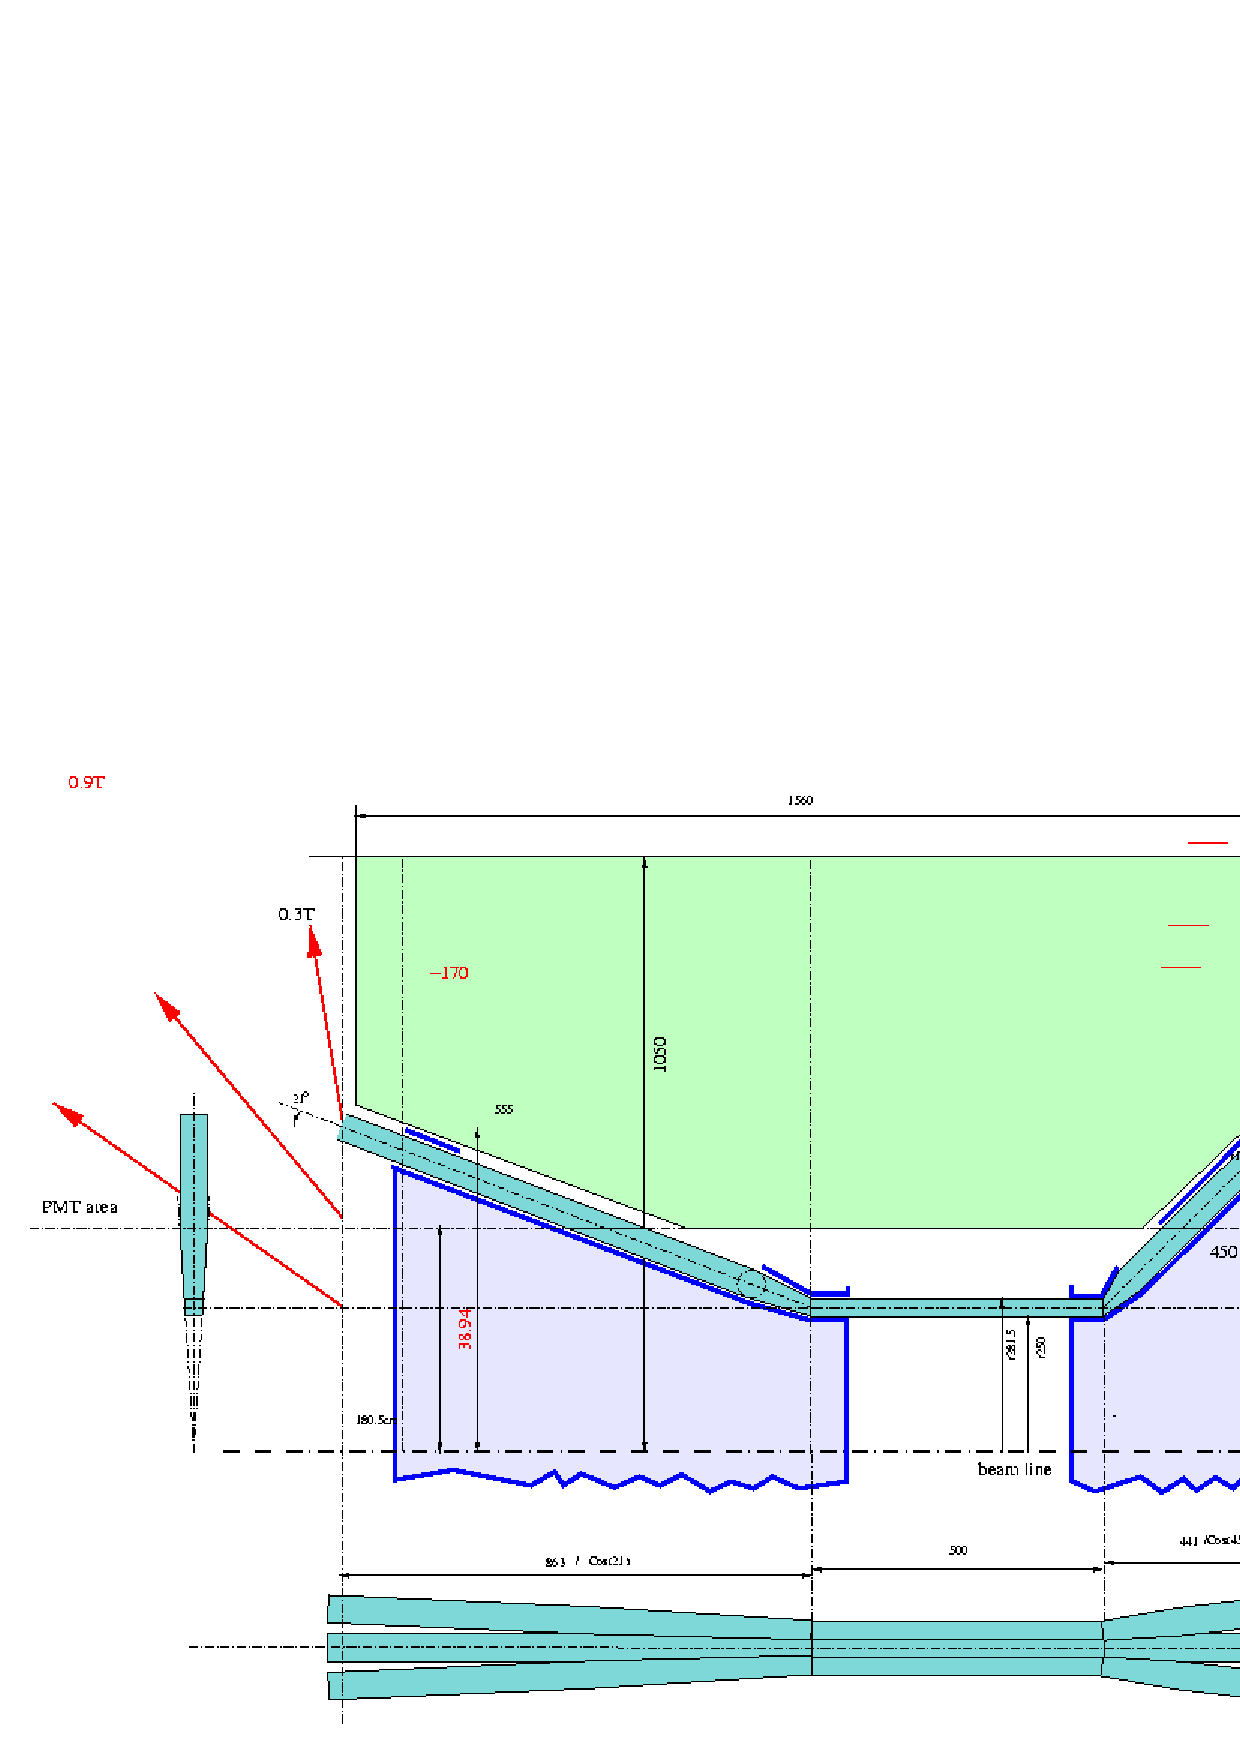
\includegraphics[height=20cm,clip=true,bb=55 0 550  780]{JLABt0H8500.ps.gz}
\end{center}
\caption{%JLABt0H8500.ps.gz,
The design  of the CLAS12 CTOF counter with 
H8500 from Hamamatsu. Acrylic light guides are rectangular in 
cross section at the photo-cathode($49\times49~mm^2$). The length of
 the upstream/downstream light guides is $863/441~mm$, respectively.
At the scintillator end LG's, as well as  ``Bicron-408'', are 
 trapezoids in cross section. At the PMT side they are squared.
Magnetic fields are shown with vectors.
\label{JLABt0H8500}}
\end{figure}
\clearpage

\newpage 
\begin{figure}[htbp]%#16
\begin{center}
%\includegraphics[width=14cm,clip=true,bb=80 0 550  800]{/home/prof/batourine/fig/bentlg03.ps.gz}
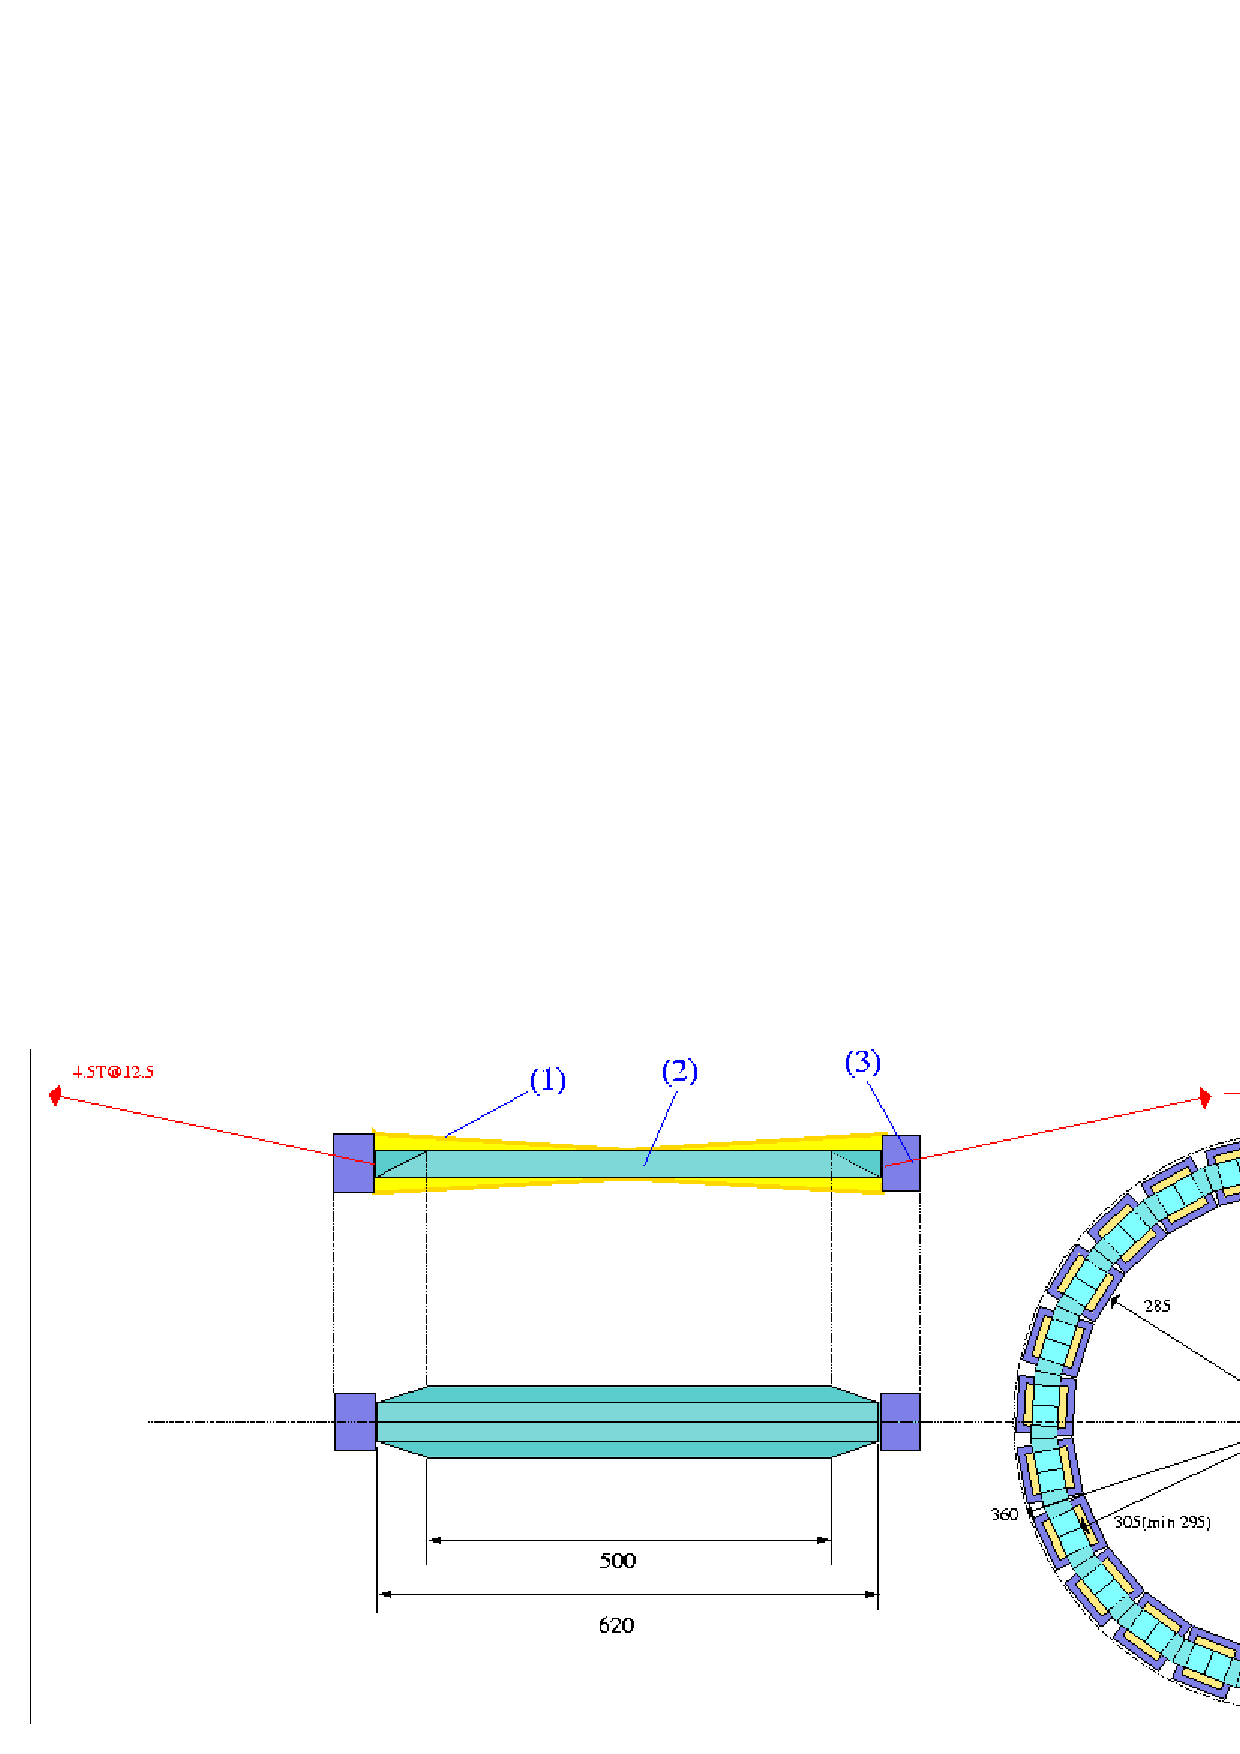
\includegraphics[height=14cm,clip=true,bb=55 30 550  820]{JLABt0H85011.ps.gz}
\end{center}
\caption{%JLABt0H85011.ps.gz,
General view of the CLAS12 CTOF counter with MCP PMs 85011 from Burle.
(1)mirror film,(2) two adjacent scintillators,(3)-Burle85011 multi-anode assembly.
\label{JLABt0H85011}}
\end{figure}
\clearpage


\begin{figure}[htbp]%#17
\begin{center}
%\includegraphics[width=14cm,clip=true,bb=80 0 550  800]{/home/prof/batourine/fig/bentlg03.ps.gz}
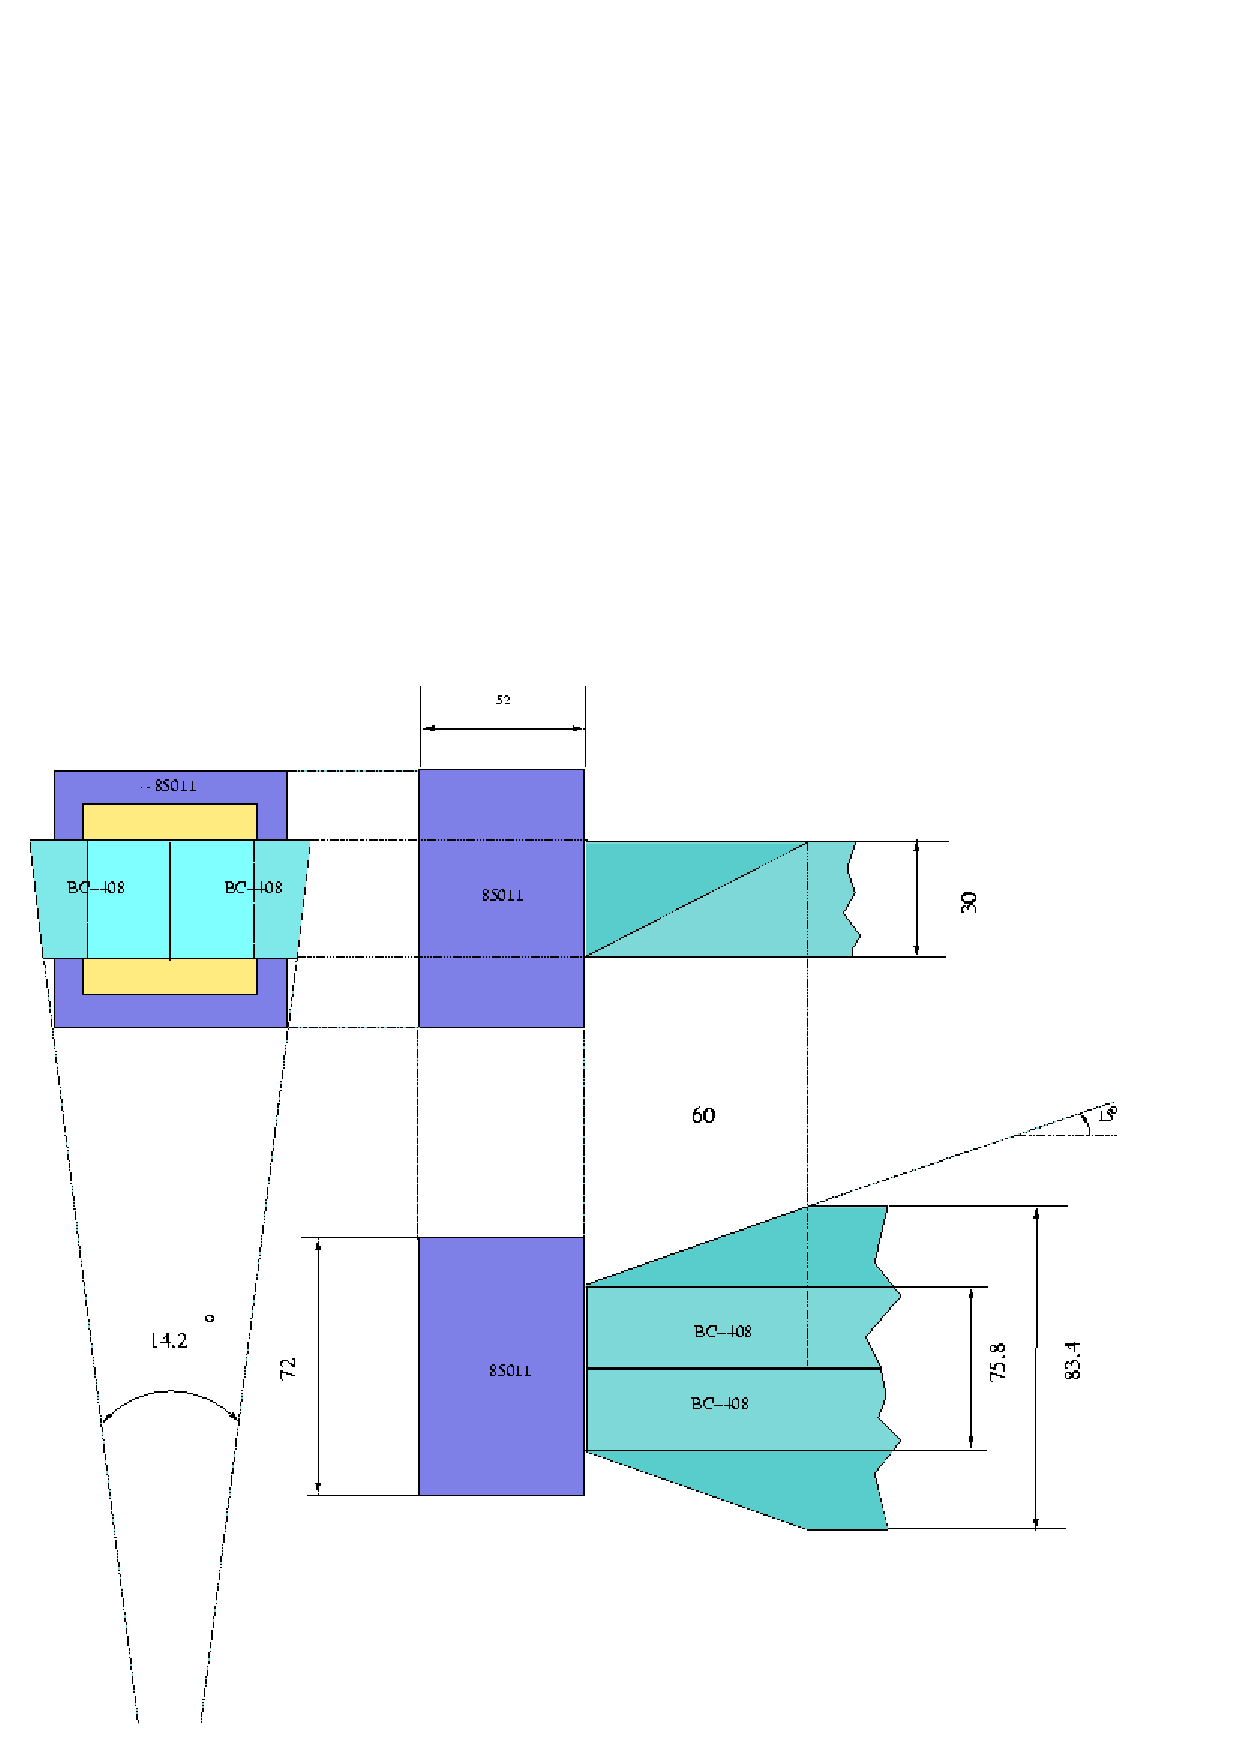
\includegraphics[width=14cm,clip=true,bb=0 0 620  700]{JLABH85011.ps.gz}
\end{center}
\caption{%JLABH85011.ps.gz,
The closer view of  the CLAS12 CTOF counter with MCP PMs 85011 from Burle. 
\label{JLABH85011}}
\end{figure}
\clearpage


\begin{figure}[htbp]%#18
\begin{center}
%\includegraphics[width=14cm,clip=true,bb=80 0 550  800]{/home/prof/batourine/fig/bentlg03.ps.gz}
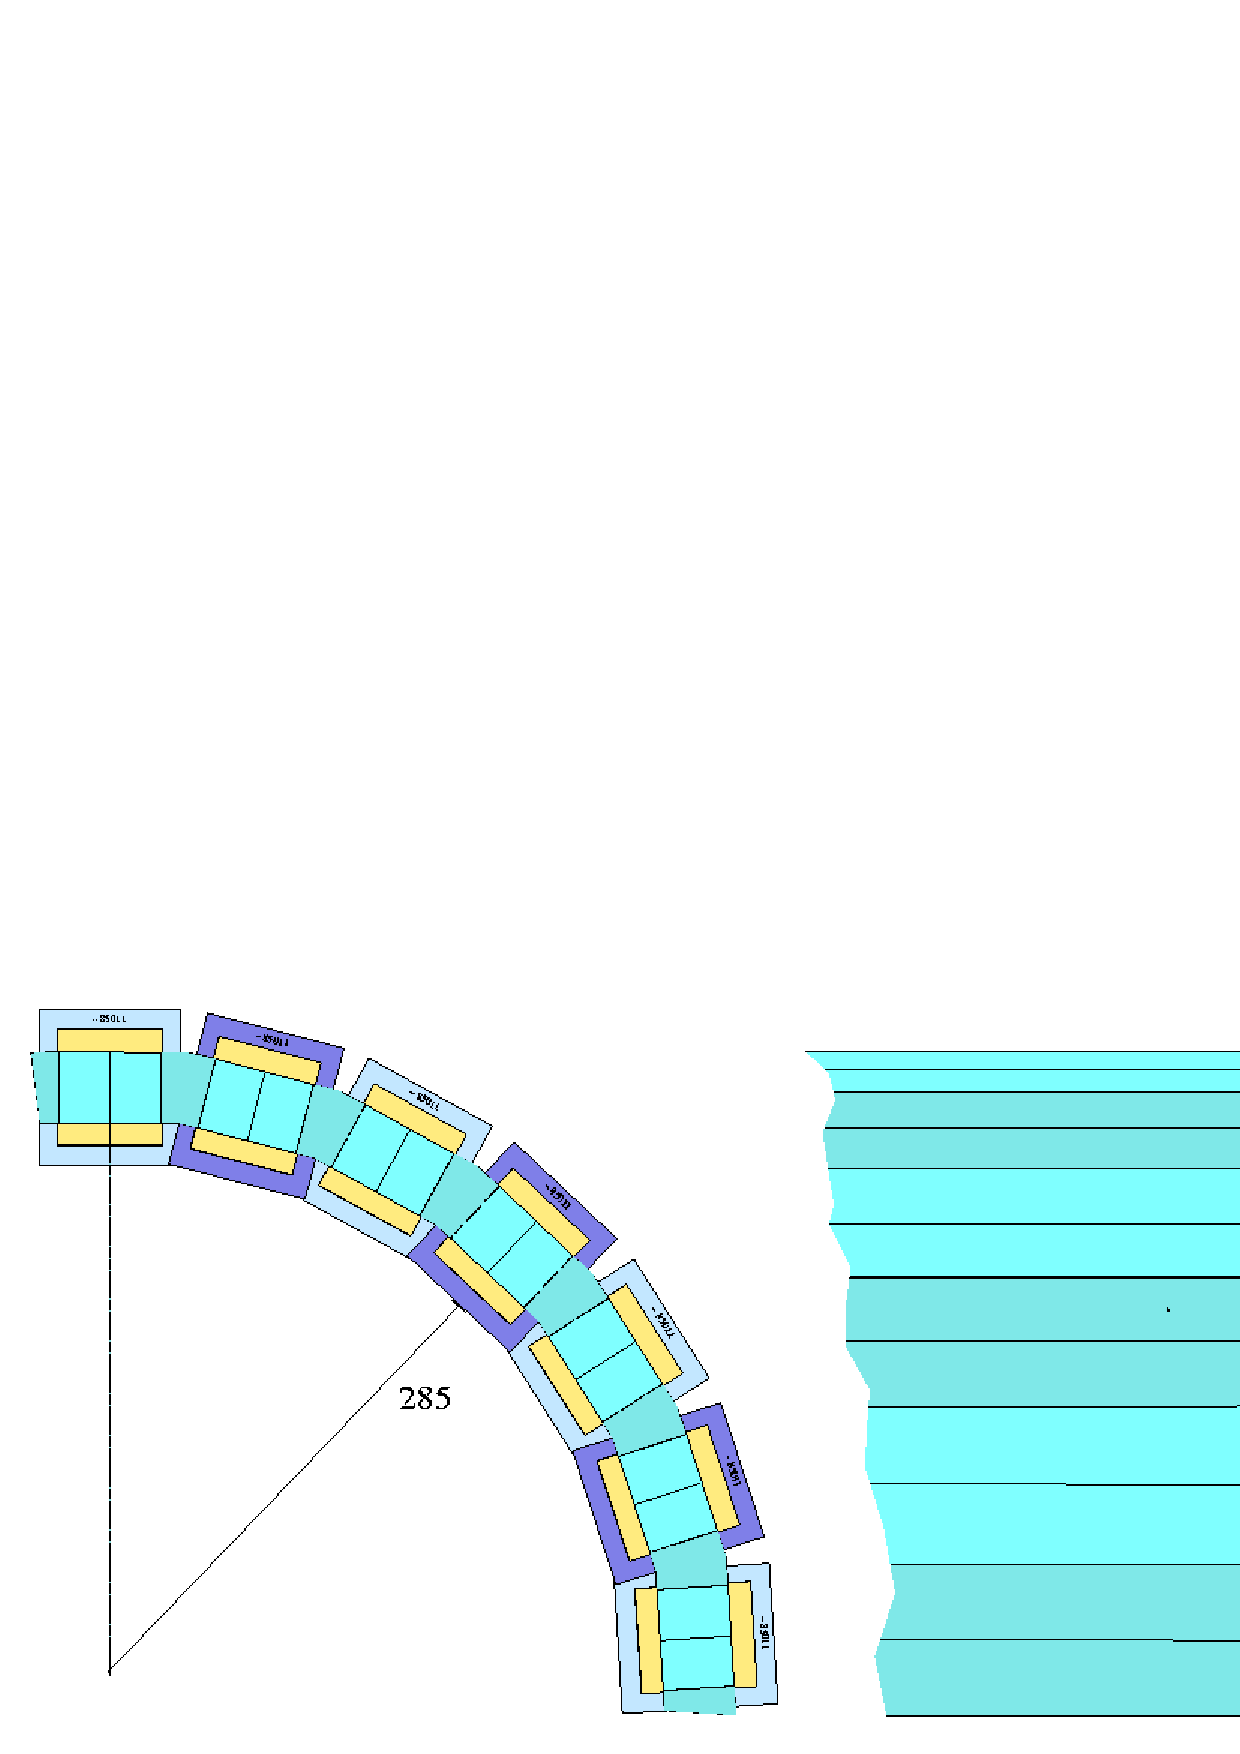
\includegraphics[width=14cm,clip=true,bb=55 30 550  820]{JLABH85011-1.ps.gz}
\end{center}
\caption{%JLABH85011-1.ps.gz,
Staggering CTOF counters with MCP PMs 85011 from Burle. 
\label{JLABH85011-1}}
\end{figure}
\clearpage

